%!TEX root = thesis.tex
\chapter{Thermal Transport in Nanowires and Thin-Films}\label{chap:predictive}
\section{Introduction}\blfootnote{Portions of this chapter have originally been published in \cite{ownNW} ``Impact of Phonon Surface Scattering on Thermal Energy Distribution of Si and SiGe Nanowires" (2016), \textit{Scientific Reports}, Vol. 6 (25818), and in \cite{ownTF} ``Surface Scattering Controlled Heat Conduction in Semiconductor Thin Films" (2016), \textit{Journal of Applied Physics}, Vol. 120 (204305). Reproduced from \cite{ownNW} under a CC BY 4.0 License, and from \cite{ownTF} with permission from AIP Publishing.}
The development of rigorous nanoscale thermal transport models requires the inclusion of the phonon-boundary scattering effects.  At the small length scales of nanostructures such as thin-films and nanowires, the physical boundaries of these structures provide a scattering mechanism for phonons. In fact, phonon surface scattering has been extensively used in the last decade to obtain significant reductions in heat conduction, and a large number of low-thermal conductivity nanostructures have been fabricated experimentally including thin-films  \cite{RN136,RN122,RN127,RN189,RN109} and nanowires \cite{RN20,RN88,NW_hochbaum,RN111,RN130,RN337,RN483}. Despite the key role played by phonon-surface interactions, these have been treated approximately in existing models. For instance, simplified kinetic theory models have relied on the Matthiessen’s rule \cite{book_Ziman} to provide an effective relaxation time to account for the reduced mean-free-paths of phonons due to boundary scattering. The intrinsic inaccuracy in the Matthiessen’s rule is the treatment of boundary scattering as an internal volumetric phenomenon (i.e., similar to phonon-phonon scattering mechanisms), while in reality the surface interaction occurs only at discrete points located at the surface. Furthermore, theoretical models have not focused on studying the phonon-surface interaction to mathematically elucidate the underlying physics rigorously. Simplified approaches have been utilized historically which do not account for all physical variables critically needed to describe this interaction, namely -- incident phonon momentum and angle as well as the surface characteristics, such as roughness and correlation length. Commonly, these approaches include the constant specularity assumption (which ignores the momentum dependence of scattering) and Ziman’s formula (which assumes all phonons to be normally incident) \cite{book_Ziman}. In addition, contrary to established approaches in optics and acoustics \cite{RN8}, the effects of rough surface shadowing on phonon surface scattering have also been unexplored in thermal phonon transport.  As a result, there is currently a need for accurately describing phonon-surface interactions in order to understand, predict, and control heat conduction processes at the nanoscale. Without achieving such fundamental understanding, it is difficult to create truly predictive models that can transition from matching with experimentally measured thermal conductivity values towards predicting transport quantities such as thermal spectra and guiding experiments to obtain rationally designed nanostructures for thermal applications.

\section{Calculating Mean-Free-Paths in Nanowires and Thin-Films}\label{sec:MFPRedModel}
The first step in obtaining predictive models is to distinguish between discrete boundary scattering events and volumetric internal scattering events. Here, we show an approach based on the a kinetic picture of phonon transport, that allows for treating boundary scattering events as discrete \cite{maldovan2011tf,RN115}. Once the accurate phononic mean-free-paths are available, they can be used to calculate transport properties, for instance thermal conductivity as shown in \Cref{eq:phonon_fourier}. In order to do so, a fundamental statistical definition of mean-free-path is used to account for the role of boundaries on phonon transport. The probability density function for phonon internal scattering in bulk as phonons propagate internally along the path length $\xi$ given by \cite{RN221},
\begin{equation}
\dfrac{dP}{d\xi}= \dfrac{1}{\ell^{\text{bulk}}}\exp(-\dfrac{\xi}{\ell^{\text{bulk}}})
\label{eq:ch2-prob}
\end{equation}
marks the starting point of this calculation. Under the assumption that the phonons in nanostructures follow similar internal relaxation rates, the change in phononic mean-free-paths \gls{mfp} in the semiconductor nanostructures stems from the introduction of boundary scattering processes. Thus, the central aim of this section is to define a framework in which the effects of boundaries can be included to evaluate phononic mean-free-paths. For illustration, we choose a thin-film to describe the mathematics behind such a calculation, while noting that the formulation holds true for any nanostructure (including nanowires) in which the geometrical distance between two successive phonon scatterings is constant. 
% Schematic 0
\begin{figure}[hbt]
	\centering 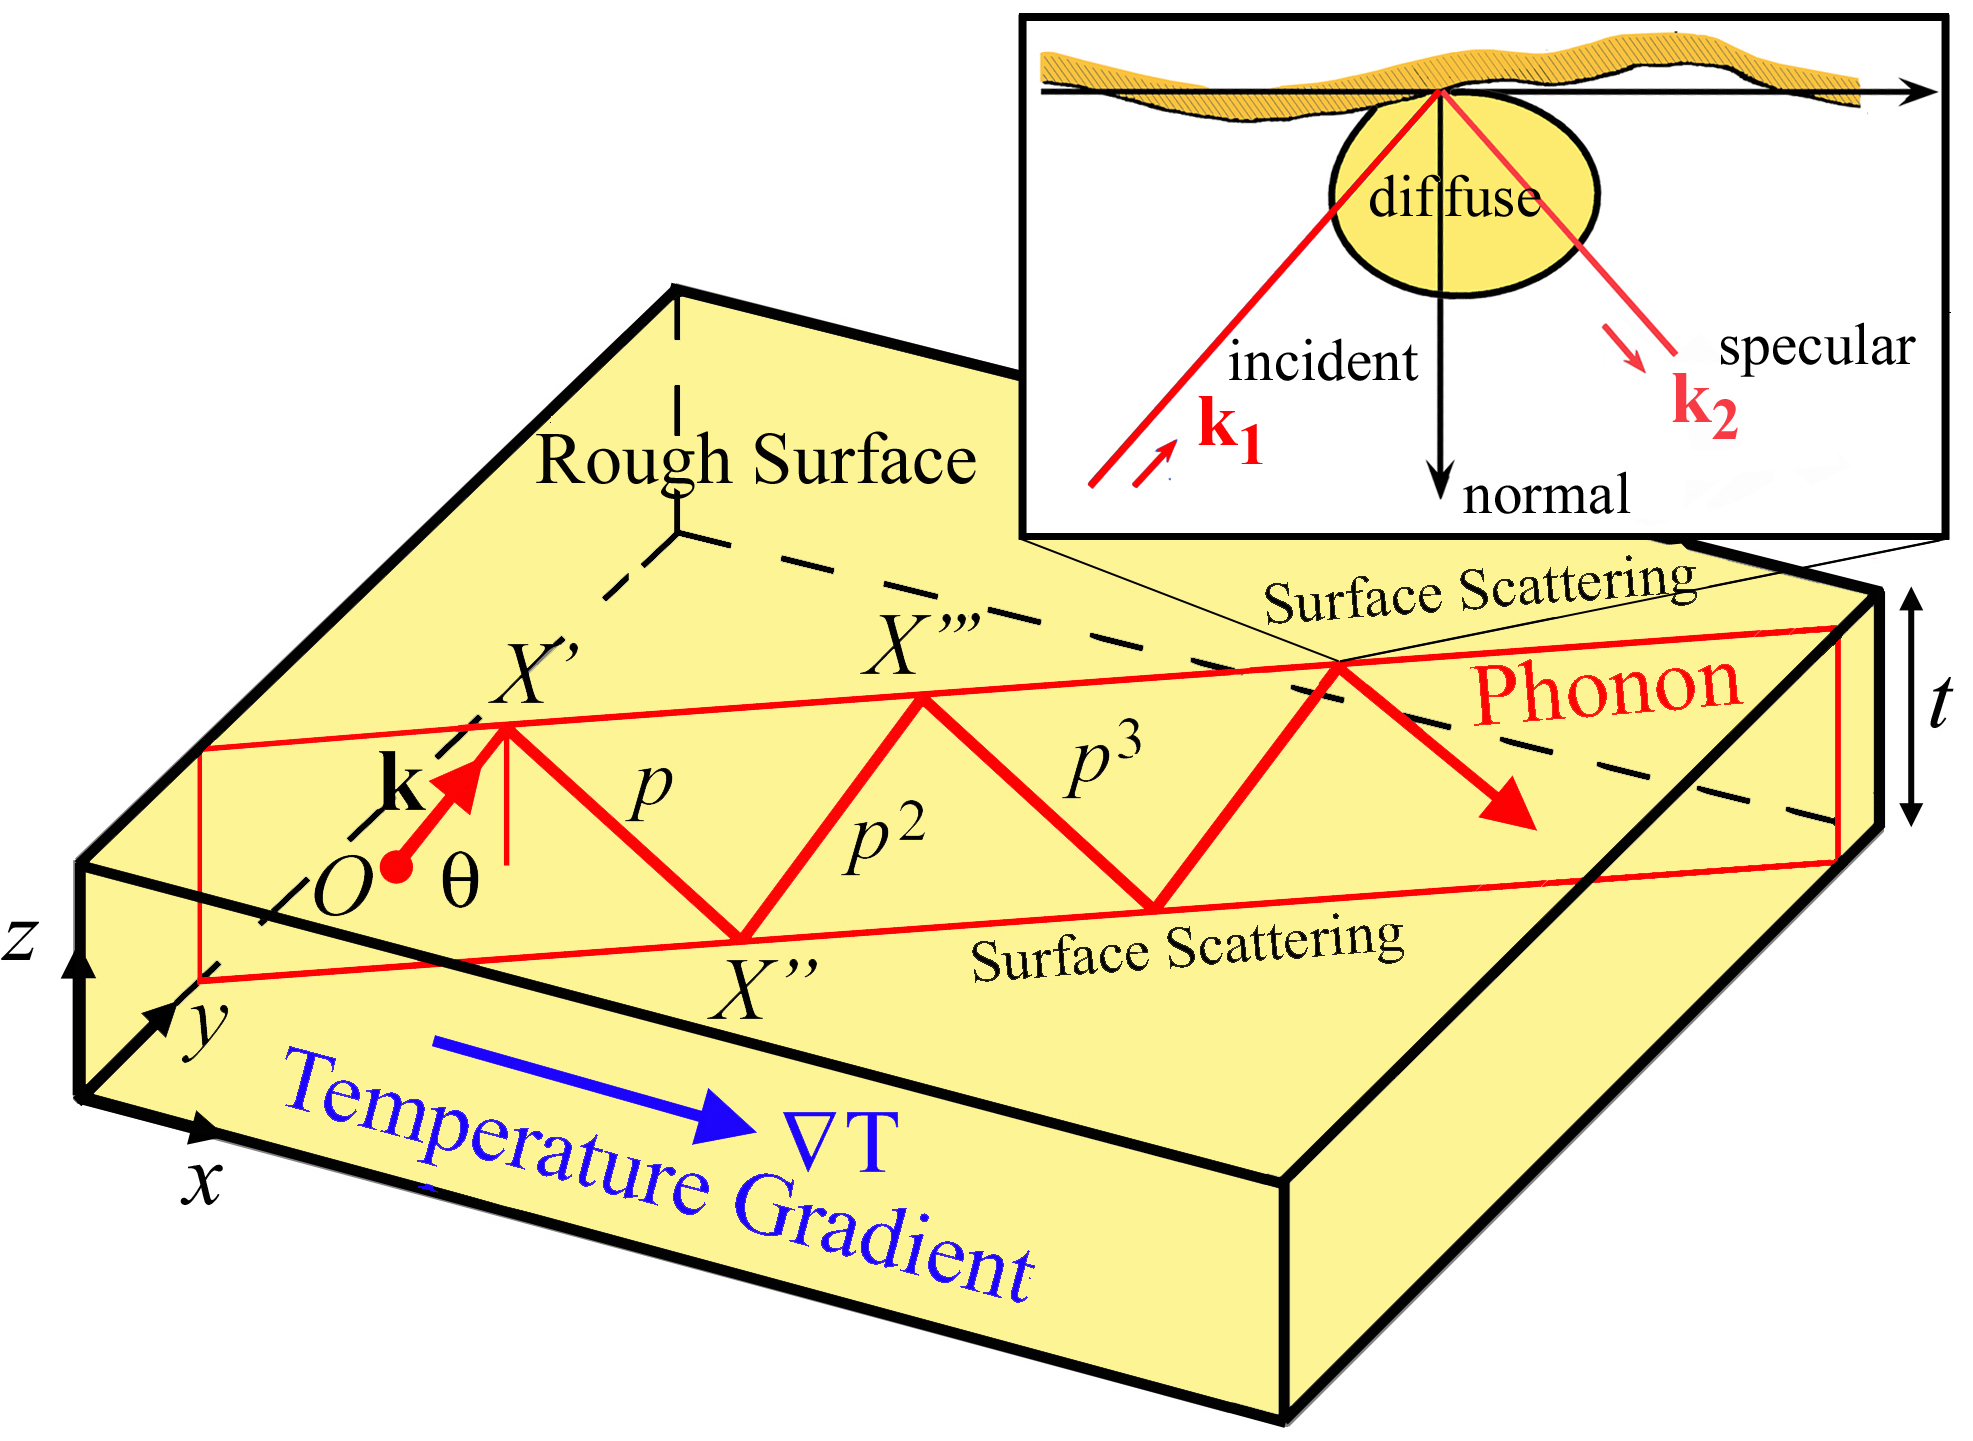
\includegraphics[width=0.95\textwidth]{/ch2/Fig1-SchematicTF.jpg}
	\caption{Schematic showing the in-plane phonon transport in a thin-film of thickness \gls{t}. The temperature gradient is applied along the $x$-direction. Phonons with wavevector \gls{k} originate at a random location O and reach the boundary at an angle \gls{theta} with the surface normal. A fraction \gls{p} of phonons are reflected specularly while the rest $1-p$ scatter diffusively at every interaction with the boundary, leading to a reduction in their mean-free-paths $\ell_{\vec{k}}$ in the thin film as compared to the bulk value $\ell^{\text{bulk}}_{\vec{k}}$.}
	\label{fig:ch2-tf_scatter_schematic}
\end{figure}
\par 
For now we lump the effect of surfaces into a \textit{specularity parameter} \gls{p} that defines the fraction of incident phonons to undergo a specular reflection, and reserve the discussion on the physical nature of the specularity parameter for \Cref{sec:BK}. During a specular reflection, a fraction \gls{p} of phonons preserve their angle of incidence \cite{book_Ziman}. On the other hand, remaining $1-p$  fraction of phonons are diffusively scattered in all directions. The diffusive scattering of a portion of phonons is central to the reduction of phononic mean-free-paths in nanostructures. For the case shown in \Cref{fig:ch2-tf_scatter_schematic}, phonons originating at point $O$ located at a distance $z$ from the upper boundary propagate at an arbitrary angle \gls{theta} with the surface normal towards the upper surface. At every interaction with the surfaces of the nanostructure, a proportion \gls{p} of incident phonons are scattered specularly, while the rest are scattered diffusively. We note that in general, phonons can encounter the interfaces repeatedly, so that in order to define their mean-free-path we use,
\begin{equation}
\ell=\int_{0}^{\infty}\xi dP
\end{equation}
By writing $OX^{'}=\Lambda$, the contribution to the mean-free-path for phonons starting at $O$ up to the point $X^{'}$ can be written as,
\begin{equation}
\ell^{{OX^{'}}}=\int_{0}^{\Lambda}{\xi dP} + (1-p)\int_{\Lambda}^{\infty}{\xi dP}
\end{equation}
where the second term represents the diffusively scattered phonons at $X^{'}$. Subsequent propagation of specularly scattered phonons from $X^{'}$ to $X^{''}$ yields the contribution,
\begin{equation}
\ell^{{X^{'}X^{''}}}=p \Bigg( \int_{\Lambda}^{\Lambda+\Lambda^*}{\xi dP} + (1-p)\int_{\Lambda+\Lambda^*}^{\infty}{\xi dP} \Bigg)
\end{equation}
where $X^{'}X^{''}=\Lambda^*=X^{'''}=...$ , allowing us to write subsequent contributions as series. We note that the mean-free-paths are dependent on phonon wave-vectors, thus we introduce a subscript \gls{k} to explicitly indicate the dependence. By using \Cref{eq:ch2-prob} to replace $dP$ with path-length traveled and sum over the total path to obtain the mean-free-paths of phonons in thin-films and nanowires as a reduction from bulk mean-free-paths.
\begin{equation}
\ell_{\vec{k}}(z)= \ell_{\vec{k}}^{\text{bulk}} \Bigg[ 1 - \dfrac{(1-p)\exp\Big(-\dfrac{\Lambda(z,\theta)}{\ell_{\vec{k}}^{\text{bulk}}}\Big)}{1-p\exp\Big(-\dfrac{\Lambda^*(t,\theta)}{\ell_{\vec{k}}^{\text{bulk}}}\Big)} \Bigg]
\label{eq:ch2-mfp_reduced}
\end{equation}

%-----------------BK--------------------
\section{Determining Specularity Parameter: Role of Surface and Phonon Properties}\label{sec:BK}
In the phonon-surface scattering process, the properties of both the surface and the incident phonons determine the dynamics. In order to characterize surfaces, a measure of the variation from a mean plane (i.e. roughness \gls{eta}) and the distance between two roughness features (i.e. correlation length 
\gls{cl}), are used. Such a description is suitable from a practical experimental standpoint as well since a surface can only be described statistically as a point-to-point description would be nearly impossible. The incident phonon properties include the incident phonon momentum ($\hbar\vec{k}$) and the incident angle with the surface normal \gls{thetai}. When a phononic population moving under an applied gradient interacts with a surface, a portion of it can be backward scattered, i.e. reflected into the same medium, while the other can be forward scattered, i.e. transmitted, across the surface into adjoining medium. These forward and backward scattering of phonons at the surface can be specular or diffuse, whose probability depends on surface properties as well as incident phonon properties. Since our purpose is to determine the specularity parameter \gls{p} for reflection, we treat the surface as a sold-air interface. To obtain the specularity parameter, the phonon field scattered by a random rough surface and its mean power over different directions is analyzed. Such a statistical behavior of rough surfaces and knowledge of their reflection coefficients have been extensively considered in studies of electromagnetic wave phenomena and acoustics \cite{RN101,book_Beckmann}. Here, we utilize the quasi-classical Beckmann-Kirchhoff (BK) framework to obtain a relation between specularity parameter and phonon wavelength, incident angle, surface roughness, and correlation length. 
\subsection{Beckmann-Kirchhoff Surface Scattering Theory}
To utilize the BK framework, we first define a one-dimensional surface S of length 2D in the ${\hat{x}}_0$ direction that separates the two solid media. Any point on such a surface can be described using a position vector \textbf{r}, 
\begin{equation}\label{eq:ch2-1} 
\mathbf{r}=x{\ \hat{\mathbf{x}}}_0+\zeta\left(x\right){\hat{\mathbf{z}}}_0                                         
\end{equation}
% Schematic 2
\begin{figure}[hbt]
	\centering 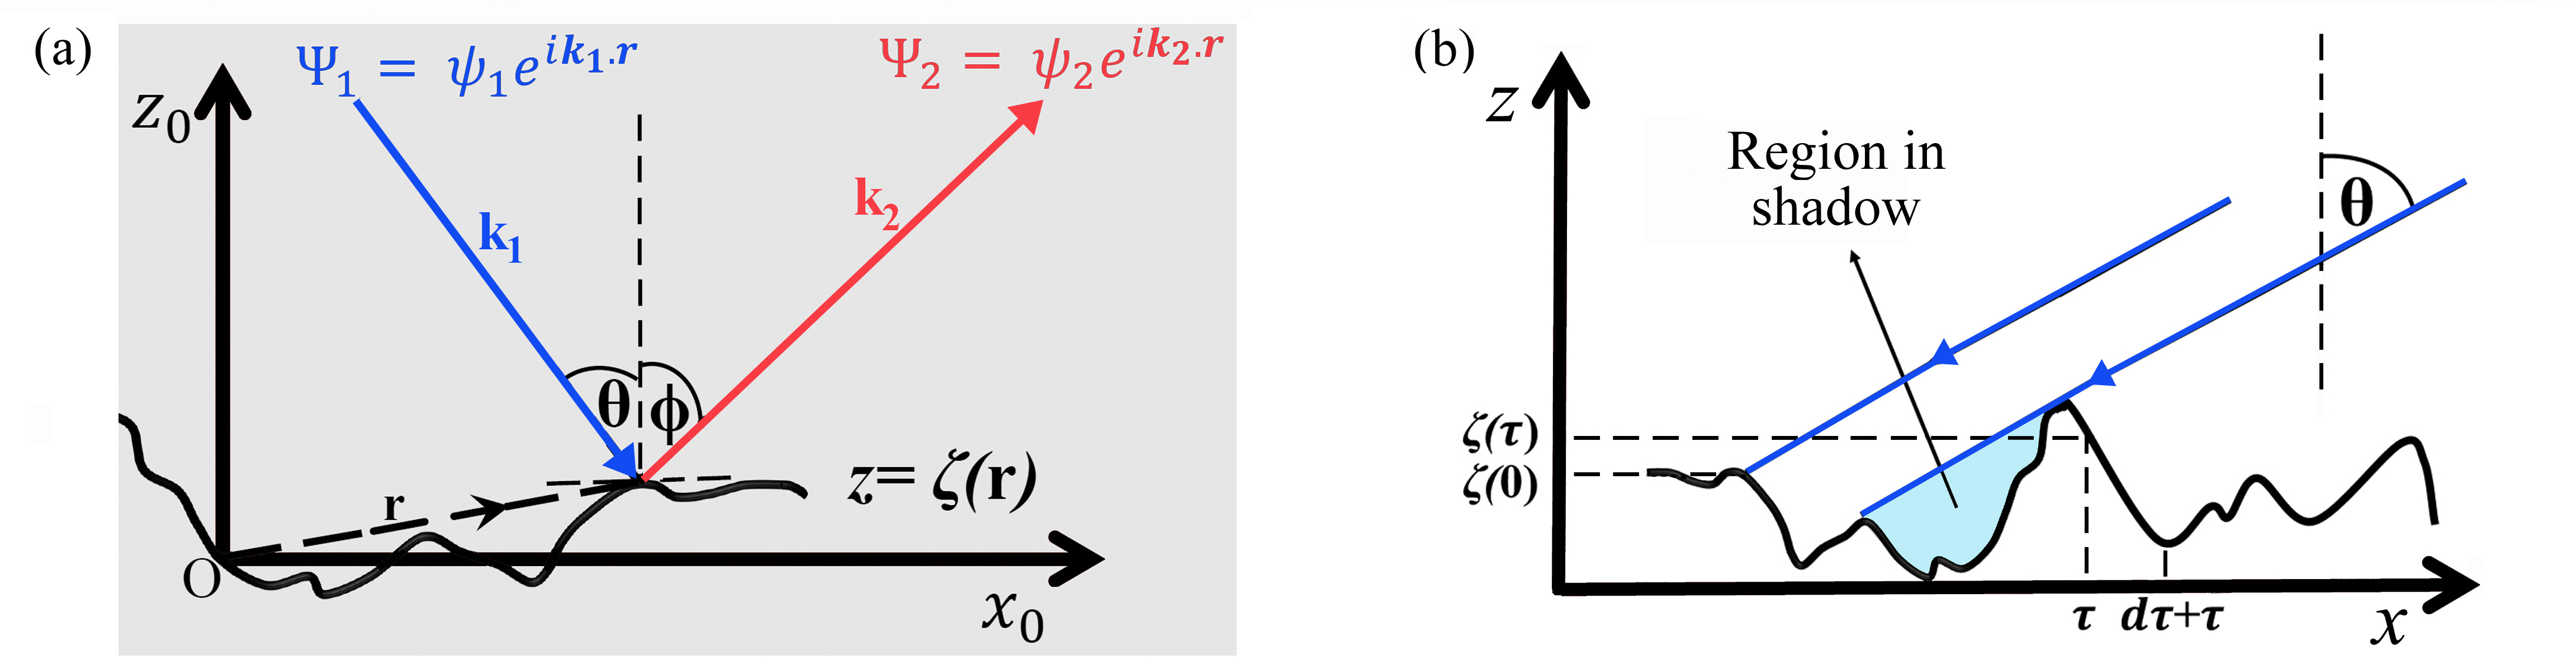
\includegraphics[width=\textwidth]{/ch2/Figure1-2.jpg}
	\caption{Schematic representation of phonon-surface interaction. (a) Incident $\Psi_{1}$ and scattered $\Psi_{2}$ phonon fields with angle of incidence \gls{theta} and scattered angle \gls{phi} from a rough surface $z = \zeta (\vec{r})$, where \gls{r} is the position vector and $\vec{k}_{1}$ and $\vec{k}_{2}$ are the corresponding wavevectors. (b) Surface shadowing. Phonons are incident with wavevector \gls{k} at angle of incidence \gls{theta} measured clockwise from the $z$ axis. Shadows are cast along the $-x$ direction reducing the surface area available for scattering.}
	\label{fig:ch2-bk_schematic2}
\end{figure}

We note that the BK method relies on the Kirchhoff approximation which requires that the surface gradients are small enough so that the field at a local tangent plane to any point on the surface approximates the field on the surface itself. Importantly, this approximation does not impose any restriction on the surface roughness (which has been a criticism of perturbation based approaches \cite{RN83}) but requires that the surface gradients are small enough so that only a minimal number of sharp features exist \cite{book_Beckmann}. Furthermore, a single scattering event from surface roughness is assumed and edge-effects are neglected. Initially, we assume that surface shadowing effects [\Cref{fig:ch2-bk_schematic2}(b)] are negligible. This is later relaxed to incorporate the effect of correlation length on specularity. In order to completely define surface properties, we assume that the distribution of surface features that obey Gaussian statistics. Under such distribution of height variations $w(z)$ around a mean plane centered at $\zeta=0$, the mathematical definition of the surface roughness can be extracted from,
\begin{equation}\label{eq:ch2-2}
w\left(z\right)=\frac{1}{\eta\sqrt(2\pi)}\exp\left(-\frac{z^2}{2\eta^2}\right)	
\end{equation}
In addition to surface roughness, a complete description of the surface also requires the information on the correlation length \gls{cl}, i.e. the distance between similar height variations. For a Gaussian distribution, the auto-correlation function enables a mathematical definition of correlation length between two repeated height variations at $x_1$ and $x_2$, and a large correlation length \gls{cl} translates to gradual slopes for the height variations. 
\begin{equation}\label{eq:ch2-31}
C\left(x_1,x_2\right)=\exp\left(-\frac{({x_1-x_2)}^2}{\mathcal{L}^2}\right)                                                  
\end{equation}
For simplification, phonons are treated as a plane-wave in this formulation with their incident field written as $\Psi_1=\psi_1e^{i\mathbf{k}_1.\mathbf{r}}$. Note that the time-dependent factor $\exp(-i\omega t)$ has been dropped since conservation of phonon energy in scattering processes is implied. Writing the Helmholtz wave equation for the total field $\Psi$,
\begin{equation}\label{eq:ch2-3}
{(\nabla}^2+k^2)\Psi=0
\end{equation}
where $k$ denotes the modulus of the wavevector \gls{k}, Green’s function theory gives the solution of the wave equation at an interior point in terms of the values of the function $\Psi$ and its normal derivative on the surface S. The scattered field $\Psi_2$ at a point of observation $X$ located at a distance $d$ from the point of incidence $(x,\zeta\left(x\right))$ at the surface is obtained using the boundary conditions, 
\begin{equation}\label{eq:ch2-4}
\Psi_{S}=(1+R)\Psi_1
\end{equation}
\begin{equation}\label{eq:ch2-5}
\left(\frac{\partial\Psi}{\partial n}\right)_{S}=\left(1-R\right)\Psi_1{\ i\ \mathbf{k}}_1.\mathbf{n}
\end{equation}
where $R$ denotes the reflection coefficient for a smooth plane and \textbf{n} is the normal to the surface. In general, $R$ may depend on the angle of incidence of the field and the physical properties of the media at both sides of the surface. However, we consider a perfectly free surface (due to the large mechanical contrast for solid-air interfaces) and therefore the reflection coefficient $R=-1$. Under the above formulation, the normalized scattered field from a one-dimensional surface yields the following expression \cite{book_Beckmann},
\begin{equation}\label{eq:ch2-6}
\widetilde{\Psi}(\theta,\varphi)=\frac{\Psi_2(\theta,\varphi)}{\Psi_2(\theta,\varphi=\theta)}=\frac{1}{2D}\sec{\theta}\frac{1+\cos{(\theta+\varphi)}}{\cos{\theta}+\cos{\varphi}}\int_{-D}^{+D}e^{i\left(\mathbf{k}_1-\mathbf{k}_2\right).\mathbf{r}}dx
\end{equation}
 where the phonons incident at angle $\theta$ and scattered at an angle $\varphi$, denoted by $\Psi_2(\theta,\varphi)$, are expressed in terms of the phonons scattered in the specular direction by a smooth, perfectly free surface with the same dimensions, i.e. $\Psi_2(\theta,\varphi=\theta)$. Using \Cref{eq:ch2-6}, we can evaluate the mean energy carried by the backward scattered phonons from the whole surface by evaluating the square of the scattered field $<\widetilde{\Psi}{\widetilde{\Psi}}^\ast>$. For the Gaussian surface under consideration here, the energy associated with the scattered field evaluates to \cite{ownNW},
\begin{equation}\label{eq:ch2-7}
\begin{split}
<\widetilde{\Psi}{\widetilde{\Psi}}^\ast>\ =\ e^{-\eta^2\left(\mathrm{k}_{1,z}-\mathrm{k}_{2,z}\right)^2}
\Bigg(\left(\frac{\sin{\left(\mathrm{k}_{1,x}D-\mathrm{k}_{2,x} D\right)}}{\left(\mathrm{k}_{1,x}D-\mathrm{k}_{2,x} D\right)}\right)^2 + \frac{\sqrt\pi\mathcal{L}}{2D}\left(\frac{1+\cos{\left(\theta+\varphi\right)}}{\cos{\theta}+\cos{\varphi}}\right)^2 \times \\ \sum_{j=1}^{\infty}\frac{\eta^{2j}\left(\mathrm{k}_{1,z}-\mathrm{k}_{2,z}\right)^{2j}}{j!\sqrt j}e^\frac{\left(\mathrm{k}_{1,x}D-\mathrm{k}_{2,x} D\right)^2\mathcal{L}^2}{4j} \Bigg)
\end{split}
\end{equation} 
%-------------------------------
% Schematic 1000000000000000000000000000
\begin{figure}[hbt]
	\centering 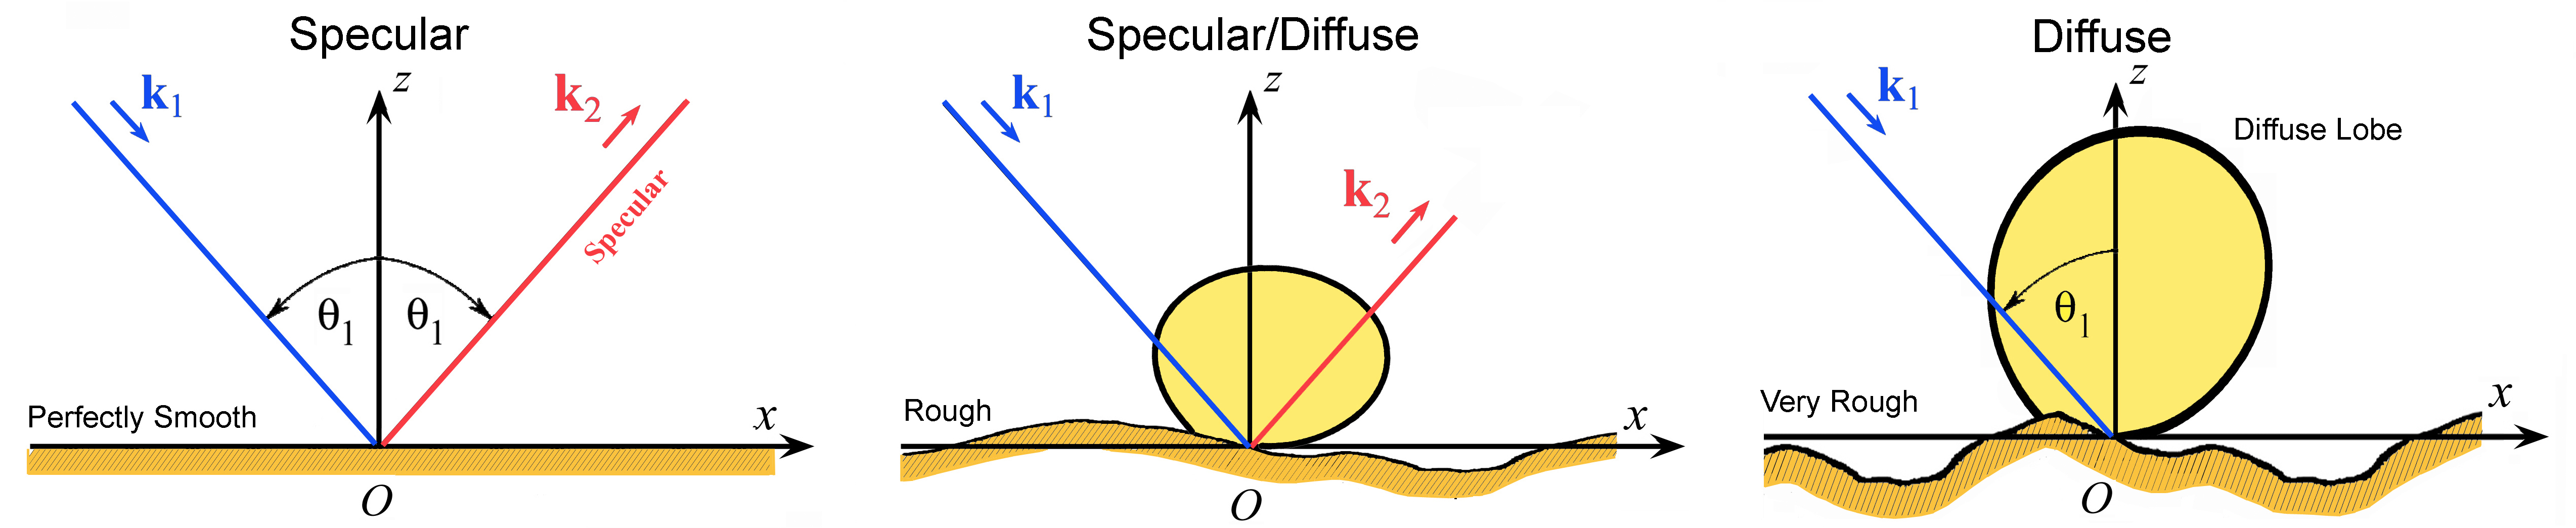
\includegraphics[width=\textwidth]{/ch2/Figure1-1.jpg}
	\caption{Schematic representation of role of roughness showing the transition from specular reflection to diffuse
scattering. \textit{Left:} Perfectly smooth surface showing perfect reflection. \textit{Centre:} Rough surface with partially
specular/partially diffuse scattering. \textit{Right:} Very rough surface exhibiting complete diffuse scattering.}
	\label{fig:ch2-bk_schematic1}
\end{figure}
%------------------
\Cref{eq:ch2-7} is also referred to as the Beckmann-Kirchhoff surface scattering model and represents a complex angular distribution of the scattered energy in a thin-film when phonons are incident at an angle $\theta$. In particular, the first term represents the specular scattering of phonons and has a sharp contribution when the scattering angle $\varphi\approx \theta$ and quickly decays at other angles. Thus, to obtain a specularity parameter \gls{p} (i.e. the proportion of specularly scattered phonons) in the limit when surface correlation length \gls{cl} is large as compared to incident phonon wavelength (i.e. $k_1\mathcal{L}\gg1$), the contribution of the first term representing the specularly scattered phonons is considered to obtain,
\begin{equation}
p=\ \exp(-\eta^2(\mathrm{k}_{1,z}-\mathrm{k}_{2,z})^2)=\ \exp(-4\eta^2\mathrm{k}_1^2\cos^2{\theta})                                     
\end{equation}

\subsection{Surface Shadowing Correction}
The Beckmann-Kirchhoff model derived above does not incorporate the phenomena of shadowing in the formulation. However, it is well understood \cite{RN86} that shadowing plays an important role in accurately predicting the scattered intensity at grazing incident angles. Shadowing is the phenomena when a portion of the surface is hidden from the incident wave by other points on the surface [\Cref{fig:ch2-bk_schematic2}(b)]. A shadowing function is introduced to account for this phenomenon mathematically and is defined as the ratio of the unscreened surface to the total surface. The shadowing correction is applied to the previously developed Beckmann-Kirchhoff scattering model by multiplying the surface area with the spatially averaged shadowing function \cite{book_Beckmann}. The initially expression obtained for shadowing was improved upon in later works \cite{RN299,RN87} and the improvement was verified by a computer generated simulation \cite{RN92}. For the case of application to heat transport, we utilize the accurate formulation presented by Wagner \cite{RN299}. 
The function $S$ to quantify the shadowing for an arbitrary point on the surface is defined as unity for points not in shadow and zero for shaded parts of the surface. The spatial averaging of this function yields the shadowing function. Considering an arbitrary point on the surface at $\tau=0$ [\Cref{fig:ch2-bk_schematic2}(b)], and define the probability,
\begin{equation}
S\left(\theta,\tau\right)=\text{Probability $\zeta\left(0\right)$ is not shaded by the surface up to $\zeta\left(\tau\right)$}
\end{equation}
allowing for definition of  $S(\theta)$ as:
\begin{equation}
S(\theta)=\lim_{\tau\to\infty} S\left(\theta,\tau\right)
\end{equation}
Based on this formulation, the shadowing function $S(\theta)$ can be expressed as \cite{RN299},
\begin{equation}
S\left(\theta\right)=\frac{\left(1+\erf\ {\left(\dfrac{0.5\mathcal{L}}{\eta}\cot\theta\right)}\right)\left(1-\exp{\left(-2B\right)}\right)}{4B}
\label{eq:shadowing-full}
\end{equation}
where
\begin{equation}
B=\frac{\exp{\left(-\dfrac{{0.25\mathcal{L}}^2}{\eta^2}{\cot}^2\theta\right)}-\left(\dfrac{0.886\mathcal{L}}{\eta}\cot\theta\right)\left(1-\erf\left(\dfrac{0.5\mathcal{L}}{\eta}\cot\theta\right)\right)}{3.545\dfrac{\mathcal{L}}{\eta}\cot\theta}
\end{equation}
For application to heat transport and models based on the specularity parameter \gls{p}, we consider a case of bistatic scattering where the scattered angle \gls{phi} lies between 0 and $\pi/2$ radians. In particular, for specular reflection the scattered angle is equal to the incident angle \gls{theta}. The shadowing function thus obtained would accurately account for the surface shadows for the Beckmann-Kirchhoff model previously described, particularly at grazing incidence angles. In particular, the bistatic shadowing function $S(\theta,\varphi)$ in the specular direction $(\varphi=\theta)$ can be expressed as,
\begin{equation}\label{eq:shadowing}
 S(\theta,\varphi=\theta)=\dfrac{\erf(\dfrac{0.5\mathcal{L}}{\eta}\cot\theta)(1-\exp(-4B))}{4B}	  	
\end{equation}
A numerical calculation of \Cref{eq:shadowing-full} is shown in \Cref{app:shadowing}. Note that the shadowing function used for calculations (\Cref{eq:shadowing}) in our heat transport model is a subset of the general function presented. Thus, the inclusion of shadowing effects enables the development of a predictive heat transport model at nanoscale, accounting for both momentum and angle dependent scattering of phonons.
%---------------------_RESULTS_----------------
\section{Predictions of Thermal Conductivity}
\subsection{Nanowires}
% NW
Looking at the literature, one of the first papers to experimentally measure thermal conductivity in silicon nanowires and show the effect of reduced diameters was by Li and coworkers \cite{RN20}. They reported the thermal conductivity of four individual nanowires of diameters \gls{dia} = 115 nm, 56 nm, 37 nm and 22 nm measured at temperatures from \gls{T} = 20 to 320 \si{\kelvin}. Since their aim was to study the impact of diameter reduction on the bulk thermal conductivity, there was no attempt to control or modify the surface roughness. The strong impact of surface roughness on nanowire conductivity was experimentally demonstrated in 2008 by Hochbaum \etal via the fabrication of rough surface nanowires of diameters \gls{dia} = 115 nm, 98 nm and 50 nm using an electroless etching (EE) method \cite{NW_hochbaum}. An attempt to quantitatively understand the lowered conductivity in rough square nanowires was subsequently made by Hippalgaonkar \etal \cite{RN191}. A further study \cite{RN131} on nanowires of diameters \gls{dia} = 50–100 nm provided insights on the range of correlation lengths. The study found that correlation length \gls{cl} ranged from 5–15 nm with average value of 9.6 nm. A later study \cite{RN67} used such etching technique for diameters \gls{dia} = 110–150 nm and gained control over the roughness of the nanowires by controlling the etching time. Such method of study was further advanced \cite{RN130} by reducing the etching rates from 100 nm/s to 0.5 nm/s and nanowires with lower roughness \gls{eta} = 1–2 nm but a similar \gls{cl} of 4–10 nm were reported. It is essential to view all this data together to truly comprehend the complexity of the problem of heat transport in silicon nanowires as shown in \Cref{fig:ch2-nwdatadump}. The experimental points lie in a region with upper and lower boundary determined by the data-sets of Li \etal and Hochbaum \etal respectively. The data visualization leads us to believe that at the current level of theoretical understanding, fabrication methodology and experimental measurement techniques, future results on reduced thermal conductivity by rough surface nanowires will continue to lie within this region. Although it is well accepted that increased roughness should lead to decreased thermal conductivities, this trend cannot be explicitly drawn from the data in the figure. This can be viewed as a complexity of the problem and shows the importance of improving the current level of theory, in addition to the need for precise and accurate measurement techniques of surface parameters (roughness, correlation length) as well as thermal conductivity, which is currently an intense research area in experimental works. In contrast to silicon, the same level of depth is not present in the case of Si-Ge alloyed nanowires. Most widely used SiGe dataset is from the work of Kim \etal \cite{RN111} and Lee \etal \cite{RN520}. However, like the initial studies on Si nanowires, there was no attempt made to quantify the surface characteristics.
%---Fig--
\begin{figure}[hbt]
	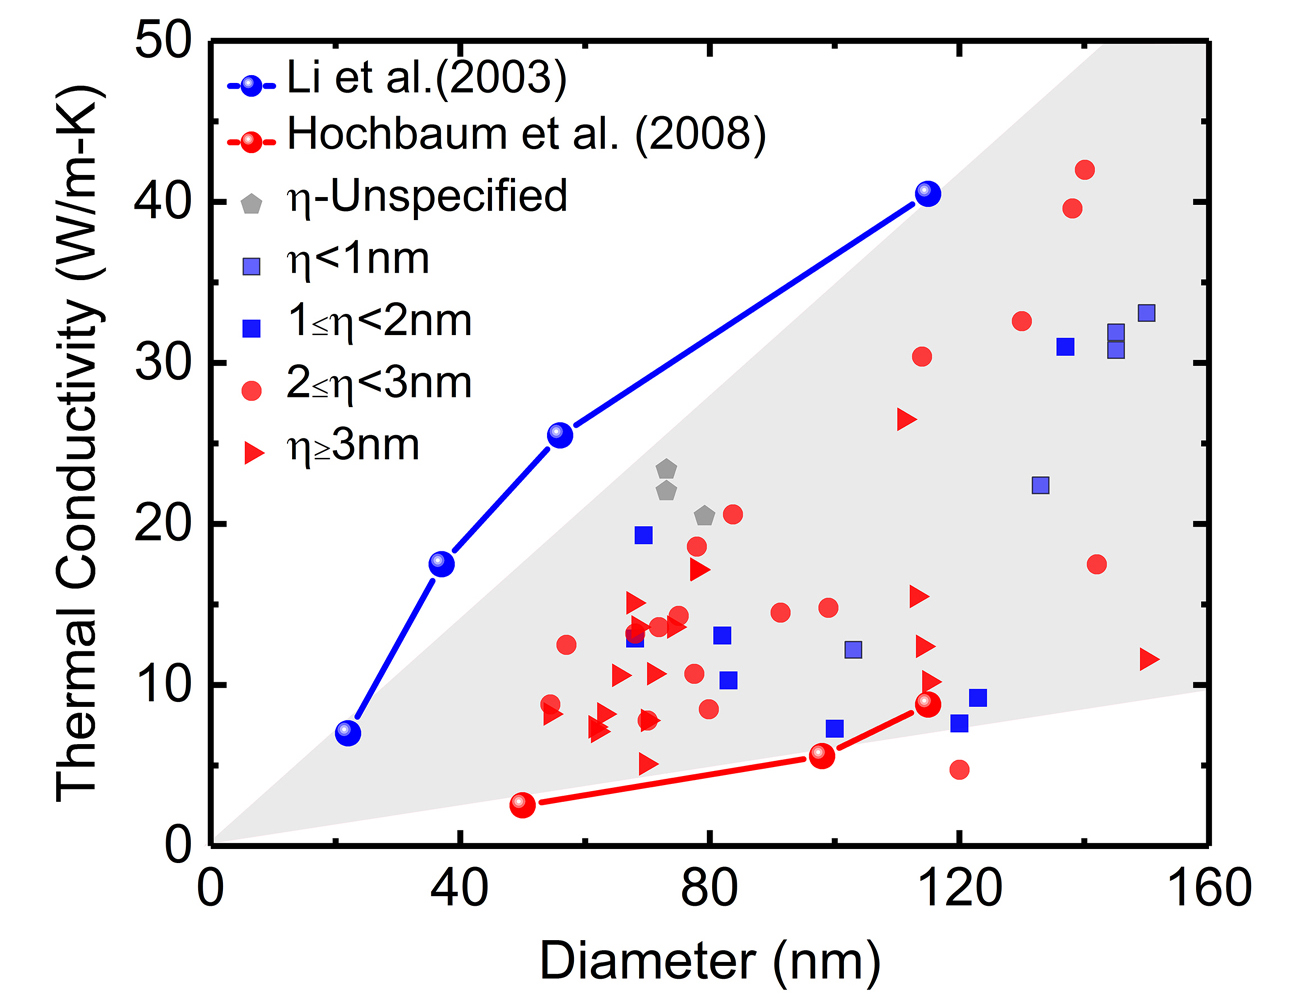
\includegraphics[width=\textwidth]{/ch2/Figure-NW-data.jpg}
	\caption{Current state of room temperature thermal conductivity engineering of nanowires. Thermal conductivity measurements by Li \etal \cite{RN20} on VLS nanowires and Hochbaum \etal \cite{NW_hochbaum} on electroless etched nanowires form an envelope around all other measurements, indicative of an experimental bound on thermal conductivity. Reprinted from ``Phononic Pathways towards Rational Design of Nanowire Heat Conduction" (2019), \textit{Nanotechnology}, Malhotra, A. and Maldovan, M. © IOP Publishing. Reproduced with permission.}
	\label{fig:ch2-nwdatadump}
\end{figure}
\todo{take permission from nanotechnology when published}
We use our surface scattering model (i.e. Beckmann-Kirchhoff formulation with shadowing and angle and momentum dependent phonon scattering) to predict Si and SiGe nanowire thermal conductivities. We find excellent agreement with experimental data-set for the un-etched nanowires of diameters 115 nm, 56 nm, 37 nm \cite{RN20} and 122 nm \cite{RN111} in \Cref{fig:ch2-nw-K}. Since no surface parameters were reported in these experiments, we assume a boundary disorder in the order of Si crystal unit cell (0.4 nm–0.6 nm) and a large enough correlation (10\gls{eta}), compared to those described in etching experiments above, as the wires were not roughened intentionally. Our accurate predictions in un-etched nanowires can be further seen in \Cref{fig:ch2-nw-K}(b) where using the previous assumptions about surface parameters, we also find a good comparison with the experimental values \cite{RN131}. For etched nanowires, the theoretical calculations are in agreement with experiments \cite{RN131,RN130} but the results are slightly larger than the experimental values. The inclusion of an amorphous layer \cite{RN103,RN240} at the boundary (to account for the chemically etched surfaces) is insufficient to account for this reduction. This enhanced reduction could be the result of micro-structural changes which appear as a result of the etching process, as suggested by D. Cahill \cite{RN67}. Additional strains in the silicon crystal introduced due to these changes were not included in our model. We also apply our model to SiGe alloy nanowires and found a similar agreement in \Cref{fig:ch2-nw-K}(c) with the experimental data by taking a higher value of roughness ($\sim 3\times$ Si lattice constant). This is consistent with a previous comparison \cite{RN289} which uses a boundary scattering description with $p = 0$. We note that accounting for changes in relaxation times due to mass difference of point defects \cite{RN289,RN132} and experimental measurements \cite{RN111,RN520} are very sensitive to impurity (alloy) fraction, a slight inaccuracy or mismatch in the reported defect percent against the actual fraction could account for the observed lowered conductivity. Interestingly, for both Si and SiGe nanowires, the BK model provides agreement with experimental results even at low temperatures where the minimum correlation length for strict applicability of the Kirchhoff approximation is expected to be higher. In addition, we predict the thermal conductivity of Si and SiGe nanowires as a function of diameter for different roughness and correlation lengths. The numerical predictions for Si nanowires in \Cref{fig:ch2-nw-K} show how the diameter reduction lowers the thermal conductivity due to the emergence of the non-diffusive (quasi-ballistic) regime of heat conduction where phonon-interface scattering plays an important role. The thermal conductivity is larger for longer correlation lengths, since the probability of phonons undergoing specular reflection is higher due to the larger distance between two surface features. We also predict the thermal conductivities for alloyed nanowires and the diameter dependence for \sige{0.90}{0.10} nanowires shows a similar trend as seen in Si for a quasi-ballistic regime. The magnitude of thermal conductivities in this case, however, are one order of magnitude smaller due to alloying effects. Our model with all the relevant physical parameters and surface scattering phenomena is thus able to predict the thermal conductivities of Si and SiGe nanowires. The presence of crystal strains and/or additional impurities in the samples could lead to lower thermal conductivities (as observed experimentally for etched nanowires).
%---Fig--
\begin{sidewaysfigure}[hbtp]
	\includegraphics[width=\textwidth]{/ch2/Figure-NW-K.jpg}
	\caption{Calculations from our model for (a) Unetched Si nanowires, (b) Unetched and etched Si nanowires and (c) SiGe nanowires for different diameters \gls{dia}. Comparison of the thermal conductivity as a function of temperature from our model shows agreement with experimental measurements (symbols) \cite{RN20,RN131,RN111,RN130,RN116}. (d,e) Theoretical predictions using our approach (BK method with shadowing) for nanowires of different diameters at room temperature with different surface characteristics (roughness and correlation length) for pure Si and SiGe alloys, respectively.}
	\label{fig:ch2-nw-K}
\end{sidewaysfigure}

\subsection{Thin-Films}
% TF
We next use our developed model to predict the thermal conductivities of Si thin films and compare the results with experimental measurements for a wide range of temperatures \gls{T} = 20 K–500 K and film thicknesses \cite{RN217,RN127,RN126,RN128,RN124,RN227,RN274,RN189,RN125}. Similar to experimental surface roughnesses in nanowires, we assume that the surface correlation length is generally in the order of \gls{cl} $\sim$ 10\gls{eta} and take the roughness values in the range of the dimension of the lattice unit cell are a reasonable approximation for un-etched silicon thin films. We note that recent works have assumed a completely diffusive boundary behavior as a good approximation of the surface behavior for most Si thin film samples \cite{RN208,RN217}. In \Cref{fig:ch2-tf-K} the distinction between a fully diffusive boundary and a free Si interface with \gls{eta} $\sim$ 0.5 nm and \gls{cl} $\sim$ 5 nm (i.e. 10\gls{eta}) can be clearly seen. Importantly, we show that the assumption of a fully diffusive boundary is valid only for small thin film dimensions and our accurate model is able to match completely the experimental results. We further note that the incorrect usage of the Ziman formula (with a $\pi^3$ in the exponent instead of $\pi^2$) can lead to overestimation of the scattering at the boundaries \cite{RN208}. Approximating Si nanostructure boundaries as perfectly diffusive is computationally simpler but is expected to be a reasonable assumption only for a reduced range of thicknesses. 
\par We also calculate the thermal conductivity of SiGe alloyed thin films, which are predicted to be an order of magnitude lower than Si thin films. This is the result of the added scattering for short-wavelength (or high-frequency) phonons due to the mass difference between Si and Ge. Variations in surface roughness and correlation lengths can significantly modify the thermal conductivity in these films as shown in \Cref{fig:ch2-tf-K}(c). The thermal conductivity is higher for larger correlation lengths and smaller roughness. This is explained by the fact that the probability of phonons undergoing specular reflection is higher when the surface is smooth and there is more separation between two surface features. The higher correlation length reduces the shadowing effects at the boundary, allowing a larger proportion of the surface to be exposed to phonons. As a result, using our model, precise predictions of the thermal conductivity can be made based on quantifiable surface characteristics (i.e., surface roughness and correlation lengths), which are critical physical parameters influencing thermal transport. 
\par The variation of thermal conductivity with surface roughness for different thicknesses and fixed correlation length is shown in \Cref{fig:ch2-tf-K}(d). The increase in surface roughness does not affect the thin-film thermal conductivity beyond a certain value ($\eta>$ 1.5 nm and 2 nm for Si and \sige{0.90}{0.10} thin-films, respectively) which indicates the complete onset of diffuse surface scattering. In an experimental setup, however, the roughening/etching of semiconductor surfaces may introduce additional strains or dislocations \cite{RN67} or cause the oxide layer formation along the interface \cite{RN393}, which can additionally affect the thermal conductivity.
%Figure TF K
\begin{figure}[hbt]
	\includegraphics[width=\textwidth]{/ch2/Figure-TF-K.jpg}
	\caption{Thermal conductivity predictions and comparison with experimental measurements \cite{RN274,RN189,RN127,RN126,RN217,RN128,RN124,RN227,RN125}. (a) Thermal conductivity as a function of temperature for Si and SiGe thin films of different thicknesses. Predicted thermal conductivity of (b) Si and (c) \sige{0.80}{0.20} thin films as a function of thickness for different surface conditions. (d) Thermal conductivity as a function of surface roughness for Si and \sige{0.90}{0.10} thin-films of thickness 500 nm (black squares), 100 nm (red-circles) and 20 nm(blue-triangles) at room temperature. The correlation length is \gls{cl} = 10\gls{eta}. Arrows indicate the onset of complete diffuse scattering.}
	\label{fig:ch2-tf-K}
\end{figure}
%SPECTRA SECTION
\newpage
\section{Predictions of Thermal Spectra}
\label{sec:pred_thermalspectra}
A current fundamental challenge in nanoscale heat transport is to precisely predict how much heat is carried by phonons with different wavelengths and mean-free-paths, i.e. normalized cumulative thermal conductivity or thermal spectra. The thermal conductivity accumulation function (i.e., the thermal energy distribution or heat spectra) as a function of wavelength \gls{wl} (or mean-free-path \gls{mfp}) is the proportion of the heat carried by phonons with wavelengths smaller than \gls{wl} (or \gls{mfp}), and provides the distribution of the heat among phonons with different wavelengths and mean-free-paths. Access to such thermal energy distribution would allow to explain the existence of ballistic versus diffuse regimes, phonon confinement, and wave interference effects \cite{RN362}. In recent years, significant efforts have been conducted to reconstruct the mean-free-path accumulative thermal conductivity of bulk materials via the combination of the suppression function and experimental measurements \cite{RN236,RN273,RN217,RN129}. This recently proposed experimental route to obtain heat spectra can be readily compared to DFT-based numerical calculations \cite{stokes_bulkSi_tau}. Importantly, if such deep knowledge of fundamental phonon transport properties in bulk materials is to be routinely extended to nanostructures, an accurate description of phonon surface scattering is critically needed beyond the standard assumption of complete diffuse scattering. In particular, a major research question that needs to be answered is the precise determination of the proportion of thermal phonons that are specularly and diffusively scattered at surfaces. The answer to this question has remained limited under the empirical approaches relying on overall relaxation times or using a constant value for the surface specularity \gls{p} (i.e. the proportion of specularly reflected phonons) without accounting for underlying physics of phonons and surfaces. The accurate prediction of thermal spectra using the described model incorporating both surface characteristics and incident phonon properties is the central goal of this section.
\subsection{Methodology}
In order to calculate thermal spectra as a function of frequency \gls{freq}, we apply a numerical approach where we create multiple \textit{bins} spanning 0.2 THz each. Similar bins of 10 nm and 2 nm were used for thermal spectra as a function of mean-free-path \gls{mfp} and wavelength \gls{wl}, respectively. Based on these bins, we numerically determine the wave-vectors \gls{k} for all polarizations that lead to frequencies (or mean-free-paths or wavelengths) lying in the bin. This approach of binning wave-vectors allow for limiting the calculation to desired \gls{freq} (or \gls{mfp} or \gls{wl}) ranges. The spectral contribution of phonons belonging to a particular wave-vector bin to overall thermal transport is evaluated by using,
\begin{equation}
\mathrm{Spectra} =\dfrac{\kappa_\mathrm{bin}}{\kappa_\mathrm{total}}\times 100\% = \dfrac{\sum_{\vec{k'}\in\,\mathrm{bin}} \hbar\omega_{\mathbf{k'}}\dfrac{\partial f^{BE}}{\partial T}v_{\mathbf{k'}}\ell_{\mathbf{k'}}}{\sum_{\forall\,\vec{k}} \hbar\omega_{\mathbf{k}}\dfrac{\partial f^{BE}}{\partial T}v_{\mathbf{k}}\ell_{\mathbf{k}}}\times 100\%
\end{equation}

\subsection{Bulk Si Spectra}
%Spectra Bulk
\begin{figure}[hbt]
  \centering \includegraphics[width=\textwidth]{/ch2/Figure-NW-Spectra0.jpg}
  \caption{(a) Comparisons between mean-free-path heat spectrum (normalized cumulative conductivity) for bulk Si from our calculations, first principle approaches \cite{stokes_bulkSi_tau}, and reconstruction from experiments \cite{RN273,RN129,RN217}. (b) Calculated wavelength heat spectrum for bulk Si and SiGe alloy, and (c) Calculated mean-free-path heat spectrum for \sige{0.90}{0.10} nanowire and the reconstructed spectrum using Ziman’s formula for \gls{eta} = 0.1 nm \cite{RN129}.}
  \label{fig:ch2-nw-spectra-0}
\end{figure}
\par We first predict the heat spectrum of bulk Si and SiGe materials and compare it against computationally expensive DFT calculations \cite{stokes_bulkSi_tau} and more recent experimental approaches that reconstruct the conductivity measurement into a heat spectrum as a function of phonon mean-free-path by use of a suppression function \cite{RN273,RN129,RN217}. We note the strong agreement between all approaches in \Cref{fig:ch2-nw-spectra-0}(a) enabling a prediction about the bulk silicon mean-free-path heat spectrum with certainty. Another important feature that needs to be considered is the thermal phonon wavelengths. Since the experimental reconstruction approach for the heat spectrum can provide only the mean-free-path spectra, we are restricted to compare our bulk calculations to DFT in \Cref{fig:ch2-nw-spectra-0}(b). Once again, our calculations for bulk silicon is in close agreement with DFT calculations \cite{stokes_bulkSi_tau}. In addition, we present our predictions for the heat spectrum of bulk \sige{0.90}{0.10} alloy. As mentioned previously, with the introduction of Ge atoms in the matrix, the spectrum shows a marked change towards longer phonon wavelengths (and larger mean-free-paths). It can thus be postulated that any change from a pure bulk structure (e.g. defects, interfaces etc.) affects both the thermal conductivity and the phonon heat spectrum. 
\par For the case of nanowires in \Cref{fig:ch2-nw-spectra-0}(c), the reconstructed heat spectrum as a function of mean-free-paths is available only for a \sige{0.90}{0.10} \cite{RN129}. This reconstruction is based on a Ziman formulation (normal incidence) for phonon boundary scattering which is expected to overestimate the effect of the boundaries \cite{ownNW}. Our results using the BTE formulation with the same assumptions show a close agreement with this reconstructed mean-free-path. Next, we look at the details of the thermal spectra in nanowires using our model.
\subsection{Nanowires}
Using our surface scattering model, we calculate the wavelength and mean-free-path heat spectra for Si nanowires for different diameters, surface roughness, and correlation lengths. \Cref{fig:ch2-nw-spectra-1} quantitatively shows how the introduction of rough boundaries strongly shifts the nanowire heat spectrum to shorter wavelengths and shorter mean-free-paths with respect to bulk silicon. For example, in bulk Si, the dominant heat carrying phonons (10–90\%) have a wavelength \gls{wl} $\sim$ 0.9–10 nm while in a nanowire of 100 nm diameter [\Cref{fig:ch2-nw-spectra-1}(a)], the dominant spectrum shifts to 0.6–2.5 nm range. A similar effect is seen in the mean-free-path spectrum which shows a marked shift from 0.1 \si{\micro}m–100 \si{\micro}m (bulk) to 15–200 nm (nanowire) [\Cref{fig:ch2-nw-spectra-1}(b)]. Such a spectrum shift is a direct consequence of the transition from bulk to a nanowire structure. In general, with the introduction of the boundaries, phonons with longer mean-free-paths (and larger wavelengths) can interact more strongly with the boundaries than those with shorter mean-free-paths. Since the roughened boundary provides an additional scattering mechanism, these phonons scatter more and achieve local equilibrium. The additional boundary scattering not only reduces the nanowire thermal conductivity as compared to bulk, but also strongly modifies the phonon heat spectra. \Cref{fig:ch2-nw-spectra-1} also shows the marked shift to shorter wavelengths and mean-free-paths with increasing surface roughness. By increasing the roughness from 0.5 nm to 1.5 nm, there is a shift to shorter wavelengths and smaller mean-free-paths in the thermal phonon distribution caused by the enhanced diffuse scattering.
%Spectra NW 1
\begin{figure}[hbtp]
  \centering 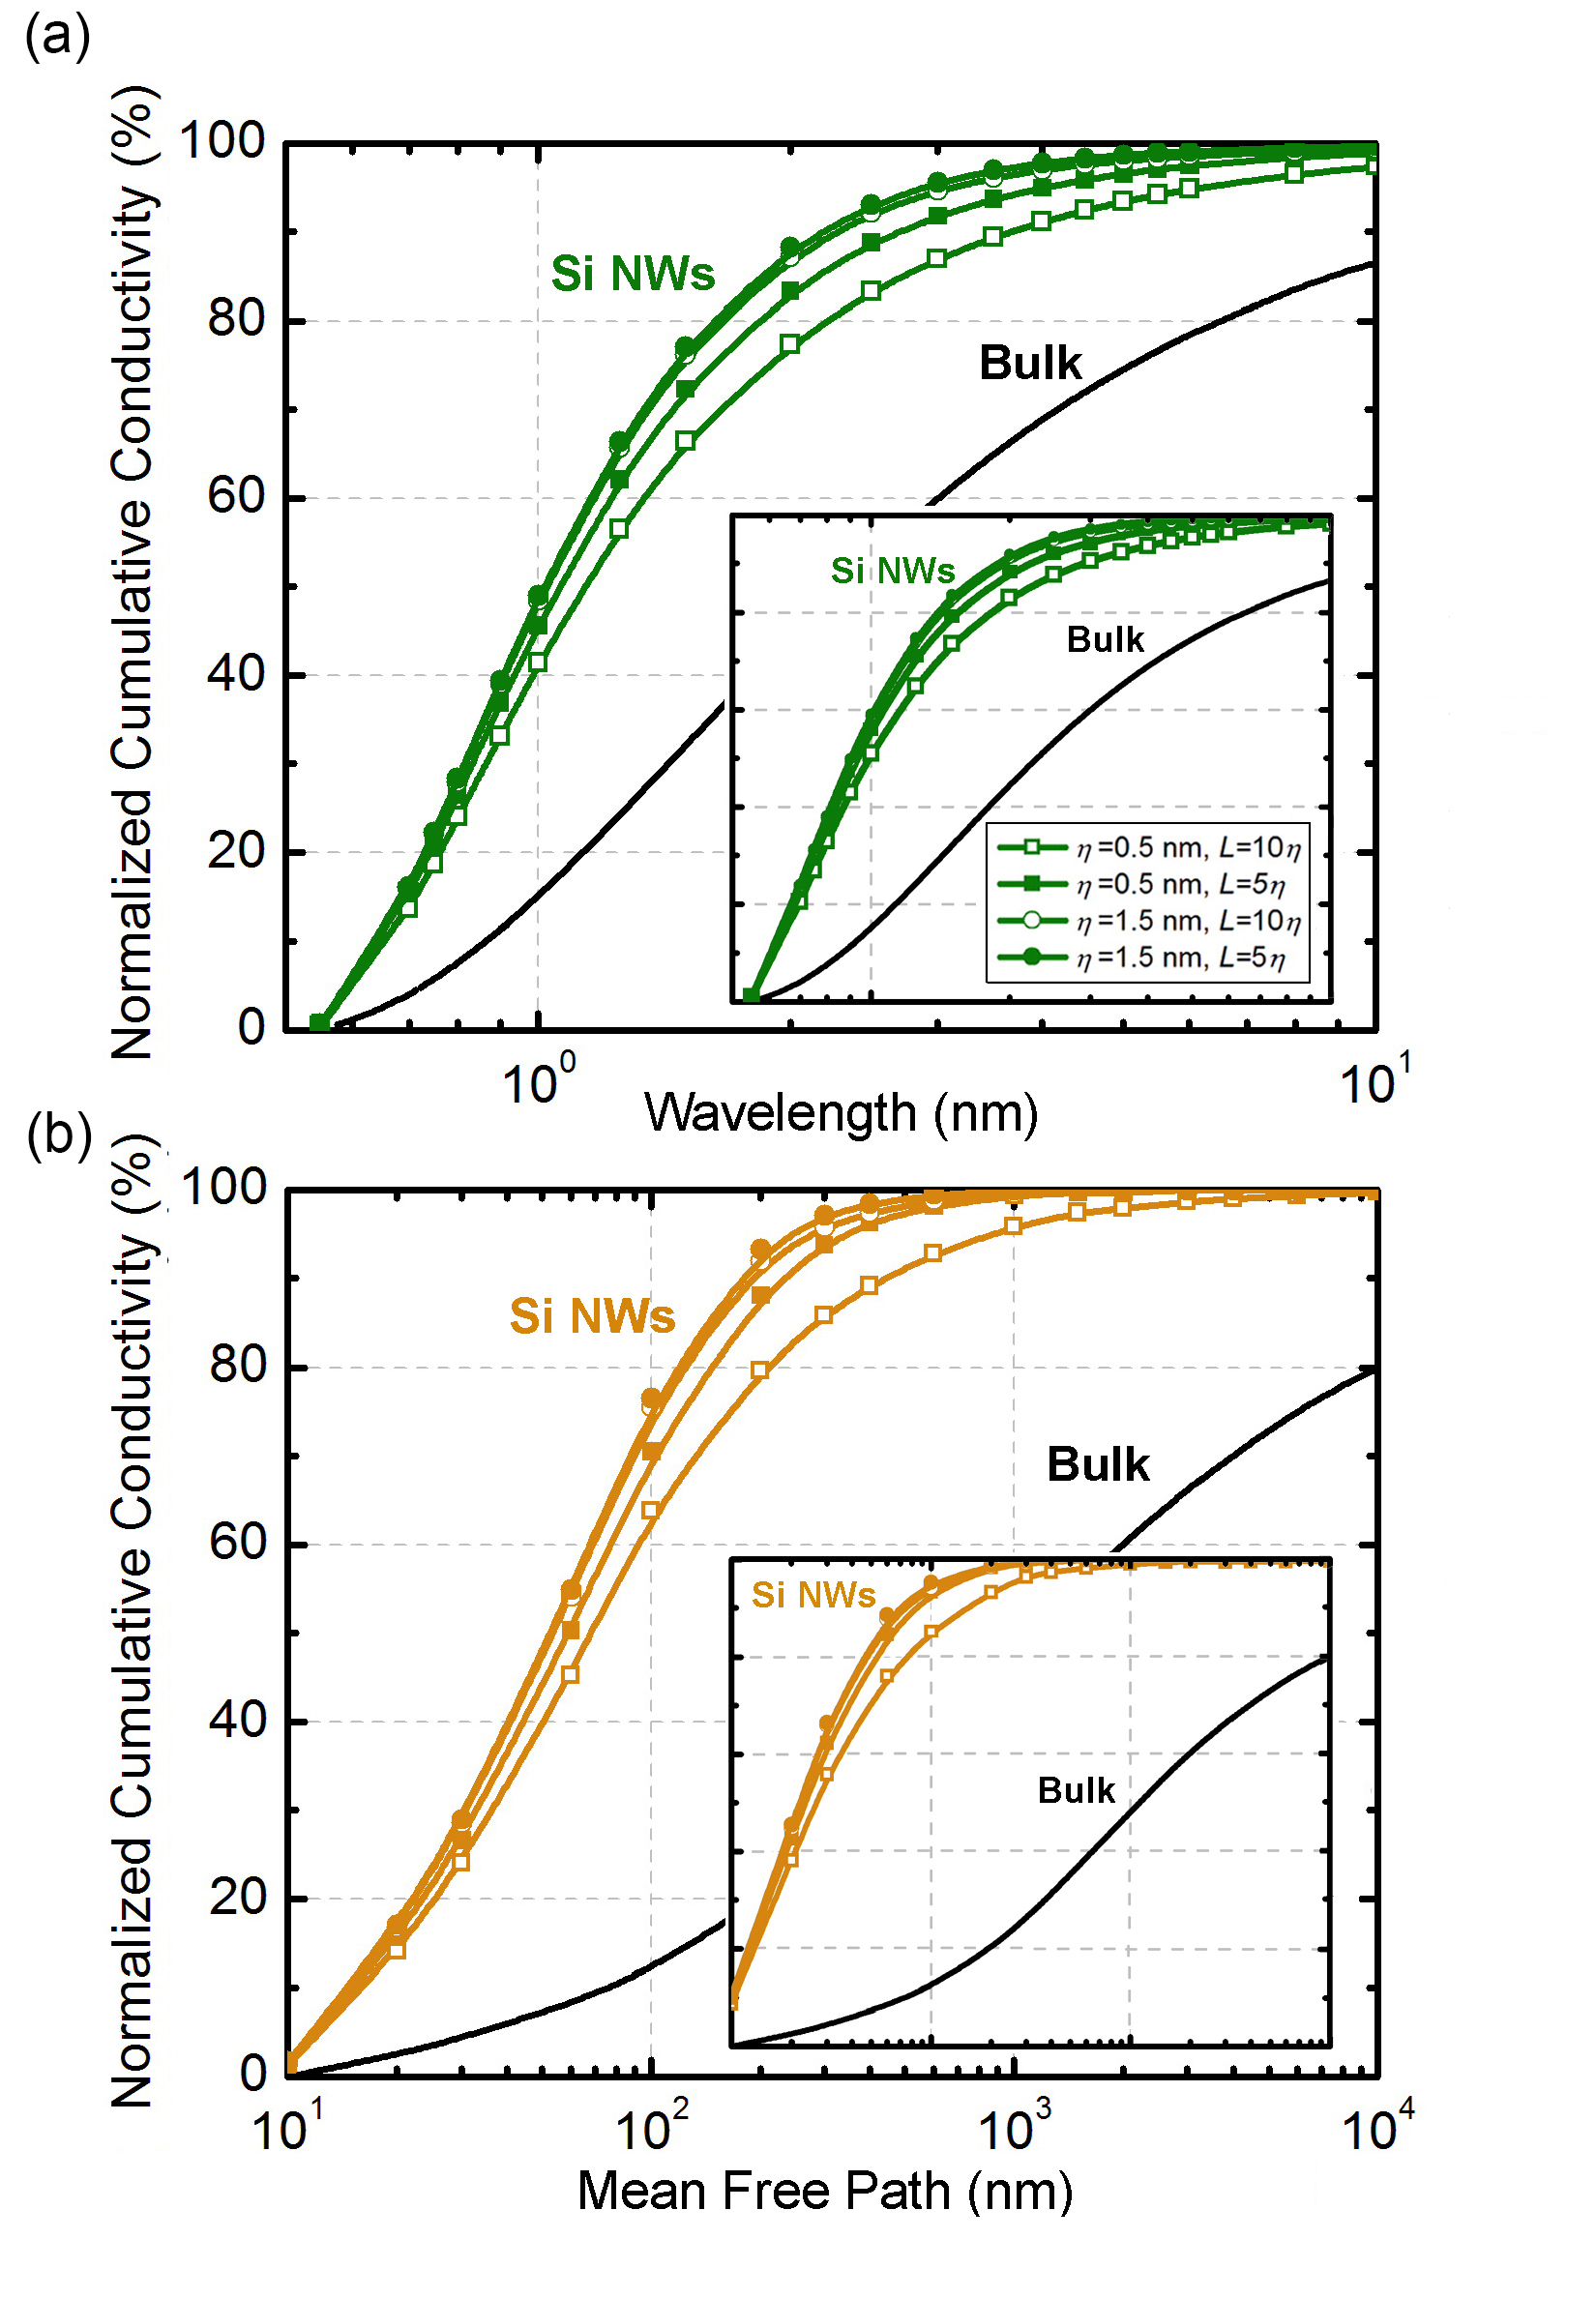
\includegraphics[width=0.85\textwidth]{/ch2/Figure-NW-Spectra1.jpg}
  \caption{Numerical prediction for heat spectra of silicon nanowires at room temperature. (a) Wavelength spectrum and (b) Mean-free-path spectrum for diameter \gls{dia} = 100 nm. Inset shows the calculations for \gls{dia} = 30 nm. Heat spectra are plotted for different roughness \gls{eta} and correlations lengths \gls{cl}. Bulk silicon spectrum is also shown as reference.}
  \label{fig:ch2-nw-spectra-1}
\end{figure} 
\par We also investigated the effects of the surface correlation lengths on the heat spectra. For a given surface roughness, a smaller correlation length enhances the impact of scattering at the boundary. This is seen as an enhanced shift in the heat spectra towards shorter mean-free-paths and smaller wavelengths (i.e. blue-shift). For example, in a Si nanowire with \gls{dia} = 100 nm and surface roughness \gls{eta} = 0.5 nm, phonons with wavelengths shorter than 2 nm carry $\sim$77\% of total heat if the correlation length is \gls{cl} = 5 nm. However, this proportion increases to 83\% if the correlation length is shortened to \gls{cl} = 2.5 nm. Similarly, in the case of the mean-free-path spectrum, phonons with mean-free-paths less than 200 nm carry 79\% of heat if \gls{cl} = 5 nm. Reducing this correlation length to \gls{cl} = 2.5 nm increases the heat carried by these phonons to 88\%. Importantly, these detailed modifications of the heat spectra cannot be predicted by approximate boundary scattering models. We note that the surface correlation length provides a statistical quantification of the distance between repeated roughness features. The frequent appearance of “hills and valleys” for a surface with small correlation length contributes towards more shadowing, modifying the probability of specular reflection. The enhanced shadowing for small correlations lengths increases the overall boundary effect causing the nanowire heat spectra to be dominated by shorter wavelength and smaller mean-free-paths. We also performed a comparison of the previous results with the spectra for a smaller nanowire (\gls{dia} = 30 nm) and found an additional shift of the spectrum to lower wavelength and mean-free-paths [\Cref{fig:ch2-nw-spectra-1}, insets]. This is consistent since the effects of boundary scattering are slightly more pronounced in a smaller diameter nanowire because a larger range of phonons can interact strongly with the nanowire surfaces.

It is important to note that, in contrast to surface scattering, the addition of mass-defects in the Si crystalline lattice in the form of Ge atoms is an effective mechanism to reduce the thermal conductivity by scattering phonons with shorter wavelengths and smaller mean-free-paths \cite{RN132,RN98}. For this reason, the dominant wavelengths and the mean-free-paths in low Ge concentration SiGe alloys are higher as compared to pure silicon. This means that while surface scattering shifts the bulk heat spectra to short wavelengths, alloy scattering shifts the bulk spectra to long wavelengths. We found that in a SiGe nanowire, where the spectra are already shifted in comparison with Si, the effect of boundary scattering is again seen by a transition to shorter mean-free-paths and wavelengths (i.e. blue-shift) [\Cref{fig:ch2-nw-spectra-2}]. This is similarly explained by the ability of the phonons with longer wavelengths (and mean-free-paths) to “see” the boundaries more effectively and have a higher interfacial interaction. An interesting property of the alloyed nanowire spectrum is the larger and broader ranges of the dominant region. If we consider the range of the middle 80\% of the heat spectrum (10–90\% of heat), the phonon mean-free-paths lie in the range of 5 nm–3 \si{\micro}m while the wavelengths are in the range of 1–20 nm. The exact value certainly depends on the roughness and correlation length of the surface under consideration. This is significantly larger and wider than the ranges seen for Si nanowires. These spectrum features are a consequence of the combined effects of alloyed scattering and boundary scattering. We note that while Ge atoms are very effective in scattering short mean-free-path (and small wavelength) phonons, boundaries are effective in interacting with phonons of larger mean-free-paths (and longer wavelengths). This leaves a larger and relatively broader “middle” range as the major conductor of the heat in the SiGe alloyed nanowires. The effects of reducing the correlation lengths via the enhanced shadowing of nanowire surface is still observed similarly to Si nanowires.
%Spectra NW 2
\begin{figure}[hbtp]
  \centering 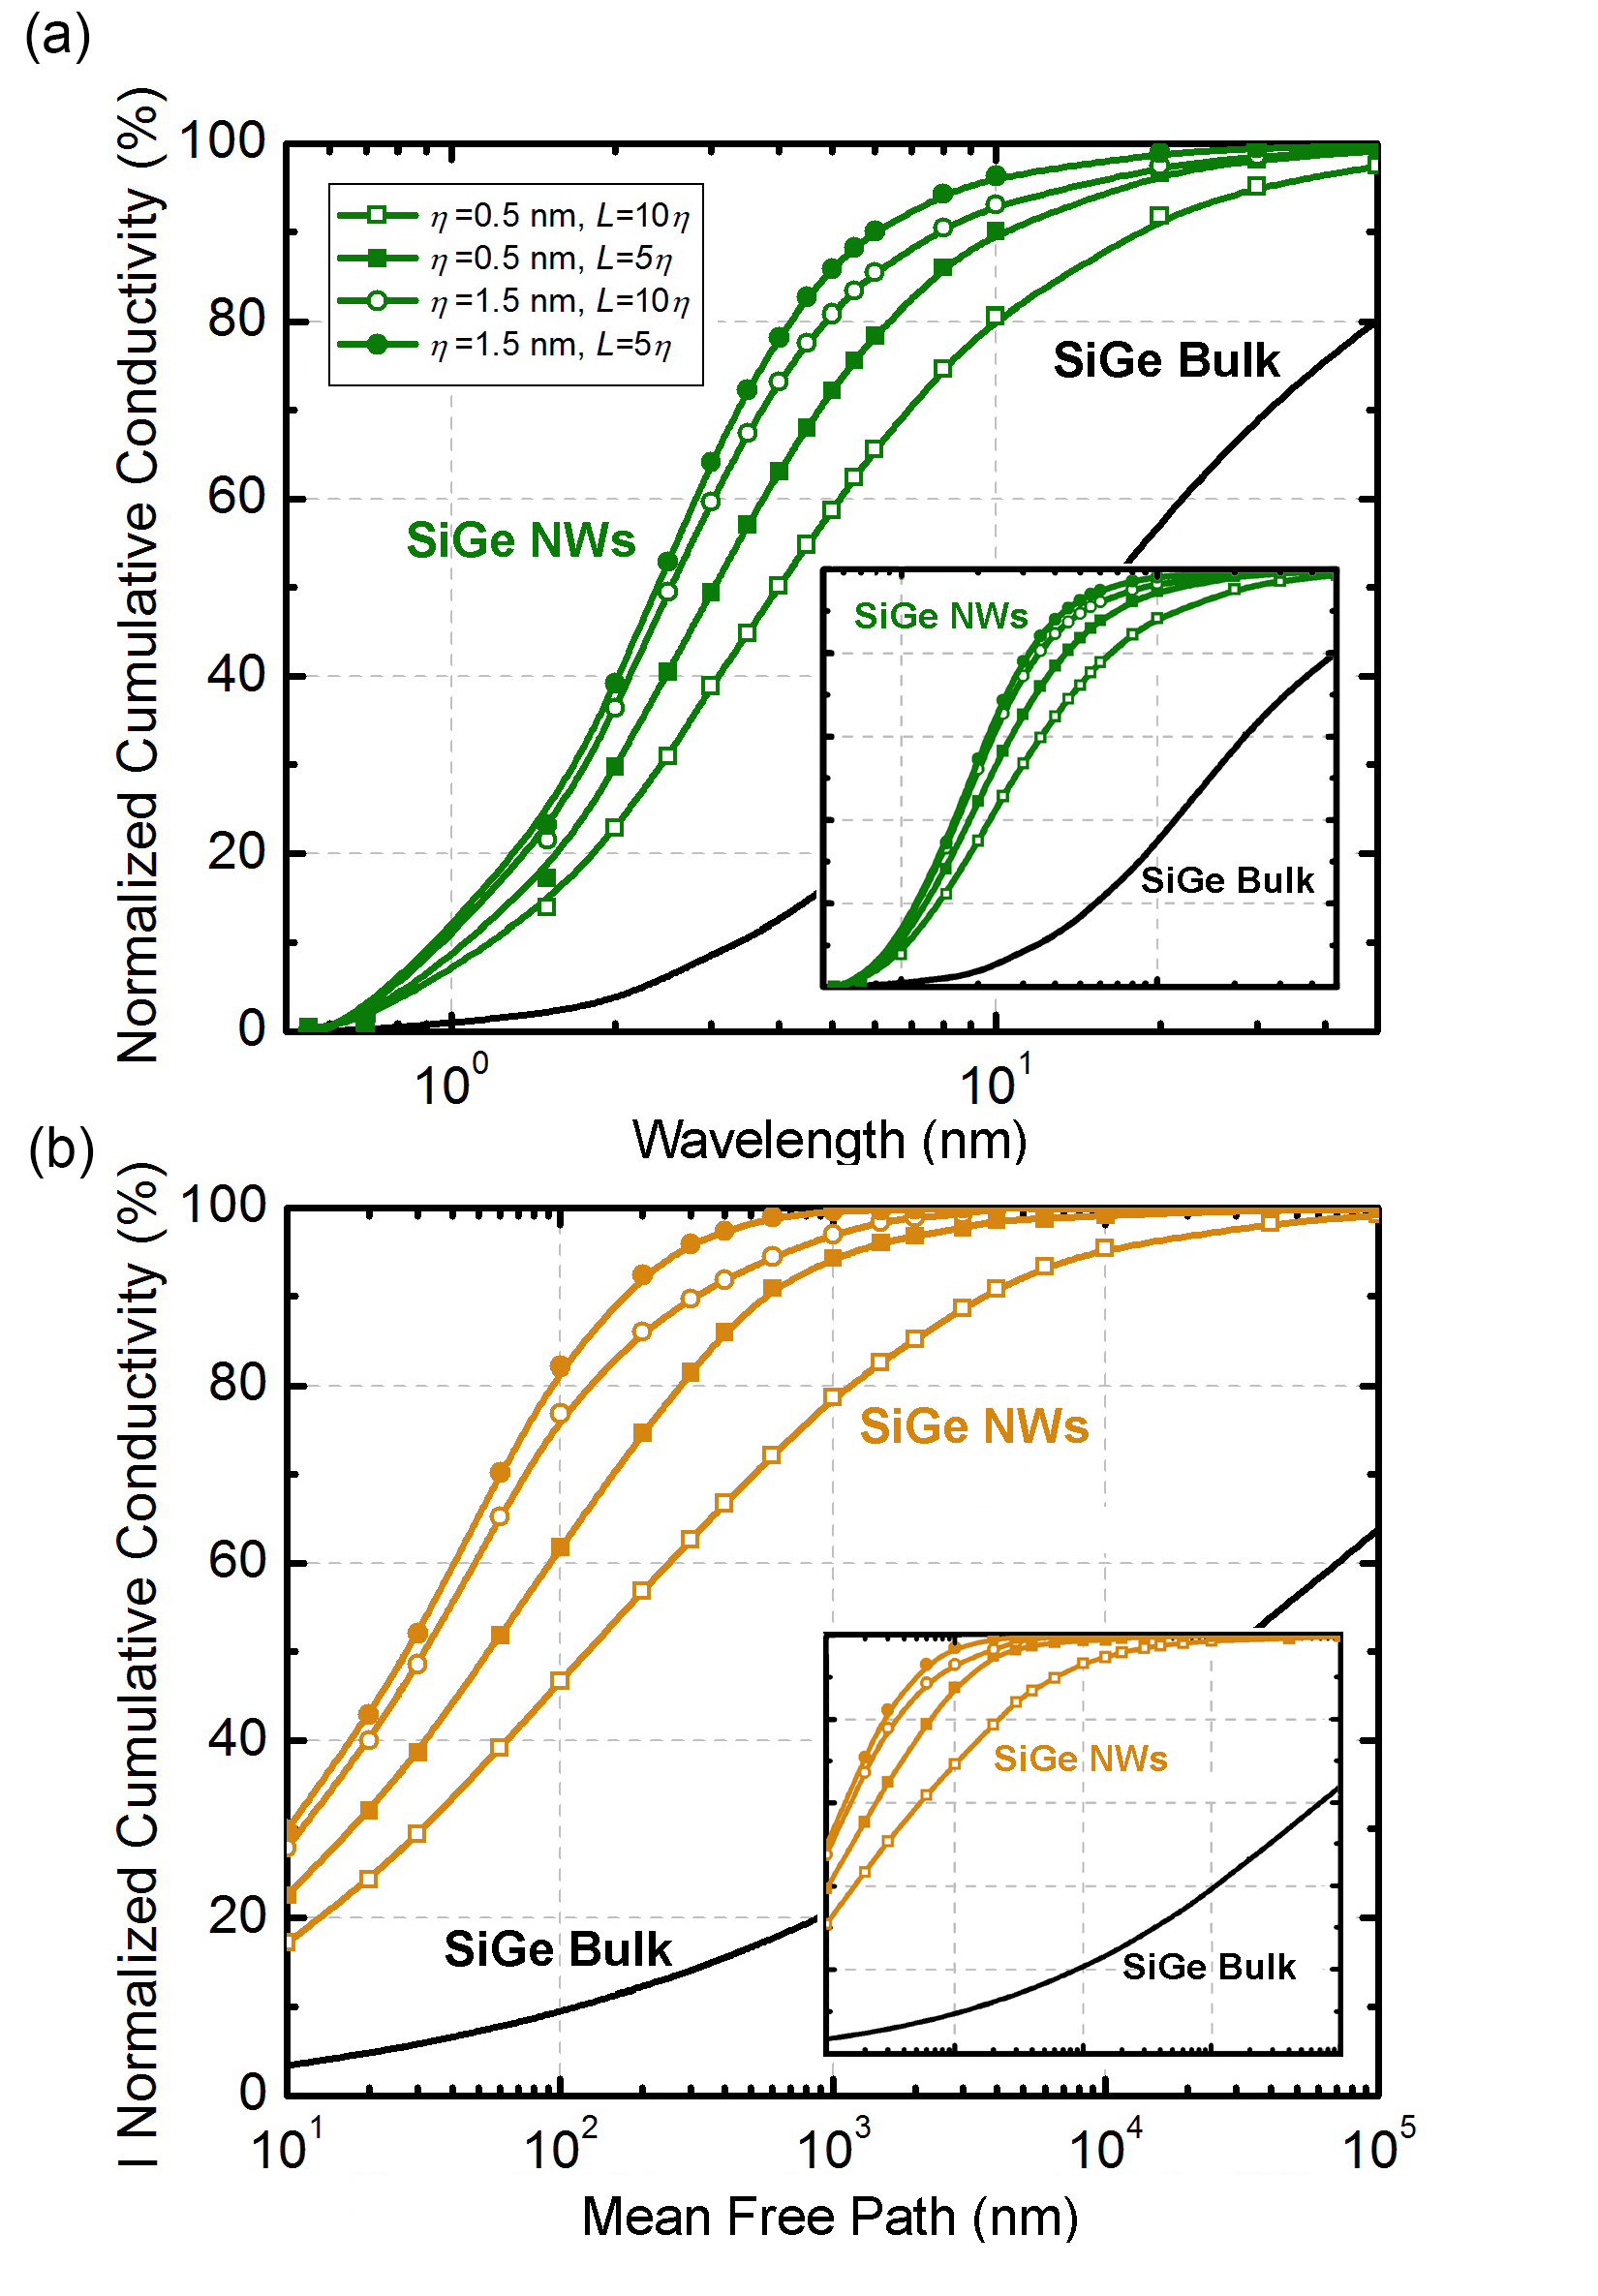
\includegraphics[width=0.85\textwidth]{/ch2/Figure-NW-Spectra2.jpg}
  \caption{Wavelength heat spectra for \sige{0.90}{0.10} alloy nanowires at room temperature for (a) \gls{dia} = 100 nm (and inset for \gls{dia} = 30 nm). (b) Mean-free-path heat spectrum for nanowire diameters \gls{dia} = 100 nm and 30 nm.}
  \label{fig:ch2-nw-spectra-2}
\end{figure}

%------TF------
\subsection{Thin-Films}
Using our model, we predict the thermal conductivity accumulation function for silicon thin films of 100 nm and 30 nm thickness and study the effects of surface roughness by choosing two vastly varying surface conditions -- a smooth (\gls{eta} = 0.5 nm, \gls{cl} = 10\gls{eta}) and a rough (\gls{eta} = 1.5 nm, \gls{cl} = 3\gls{eta}) interface, respectively [\Cref{fig:ch2-tf-spectra-1}]. We find that the introduction of different interfaces can differently modify the accumulation function to shorter wavelengths and shorter mean-free-paths with respect to bulk silicon. For example, in bulk Si, the dominant heat-carrying phonons (20\%–80\%) have a mean-free-path of 0.2 \si{\micro}m–10 \si{\micro}m (wavelengths 1–7 nm). The introduction of a smooth boundary in a 100 nm thin film, however, alters these ranges to 40 nm–420 nm (0.85–2.5 nm) and a rough interface modifies these to 35 nm–300 nm (0.80 nm–2 nm). The observed shift of the accumulation functions to shorter wavelengths and mean-free-paths is the consequence of greater diffuse surface scattering of phonons. Phonons with longer mean-free-paths can effectively interact with the rough surface, while the smaller correlation length creates a surface with enhanced shadowing. This combination of increased roughness and shortened correlation length leads to phonons with shorter mean-free-paths (and wavelengths) to become dominant thermal carriers. These trends in the accumulation function are also observed in the thinner 30 nm silicon thin film [\Cref{fig:ch2-tf-spectra-1}, insets].
%Spectra TF 1
\begin{figure}[hbt]
  \centering \includegraphics[width=\textwidth]{/ch2/Figure-TF-Spectra1.jpg}
  \caption{Numerical predictions for the thermal conductivity accumulation functions for Si and SiGe thin films at room temperature. (a) Wavelength spectrum and (b) Mean-free-path spectrum for thickness \gls{t} = 100 nm. Insets, show the corresponding calculations for \gls{t} = 30 nm. Accumulation functions are plotted for different roughness \gls{eta} and correlations lengths \gls{cl}. Accumulation functions for \sige{0.90}{0.10} alloyed thin films are also calculated as a function of phonon (c) Wavelength and (d) Mean-free-paths. Black solid lines show the bulk thermal conductivity accumulation as reference.}
  \label{fig:ch2-tf-spectra-1}
\end{figure}
\par We also consider SiGe alloy films and predict the thermal conductivity accumulation under different surface conditions. It is important to note that there is a significant modification in the bulk \sige{0.90}{0.10} energy spectra (with respect to bulk Si) due to the mass-difference scattering generated by atomically heavier Ge atoms, which are effective in scattering high frequency phonons. This results in the middle 60\% of the energy to be carried by phonons of mean-free-path 1 \si{\micro}m–500 \si{\micro}m (wavelength 6–60 nm) in bulk SiGe. For the 100 nm SiGe thin film, the additional phonon boundary scattering creates a dominant region of phonons with mean-free-paths ranging from 25 nm–1500 nm (2 nm–10 nm) for a smooth boundary and 10 nm–250 nm (1.5 nm–5 nm) for a rough boundary. Effect of temperature on the thermal conductivity accumulation function is also explored in \Cref{fig:ch2-tf-spectra-2} for Si thin film (\sige{0.90}{0.10} in inset) of thickness 100 nm with smooth (\gls{eta} = 0.5 nm, \gls{cl} = 10\gls{eta}) and rough (\gls{eta} = 1.5 nm, \gls{cl} = 3\gls{eta}) interfaces. We note that the accumulation functions are determined by two mechanisms acting on different phonon wavelengths -- increase in temperature excites short wavelength phonons, while surfaces primarily scatter large wavelength (and mean-free-path) phonons, suppressing their contribution [\Cref{fig:ch2-tf-spectra-2}(a)]. In addition, in SiGe alloys, mass difference scattering promotes large-wavelength phonons as dominant carriers, allowing the boundary scattering mechanism to act on a broader range of heat-carrying phonons [\Cref{fig:ch2-tf-spectra-2}(b)]. 
%Spectra TF 2
\begin{figure}[hbt]
  \centering 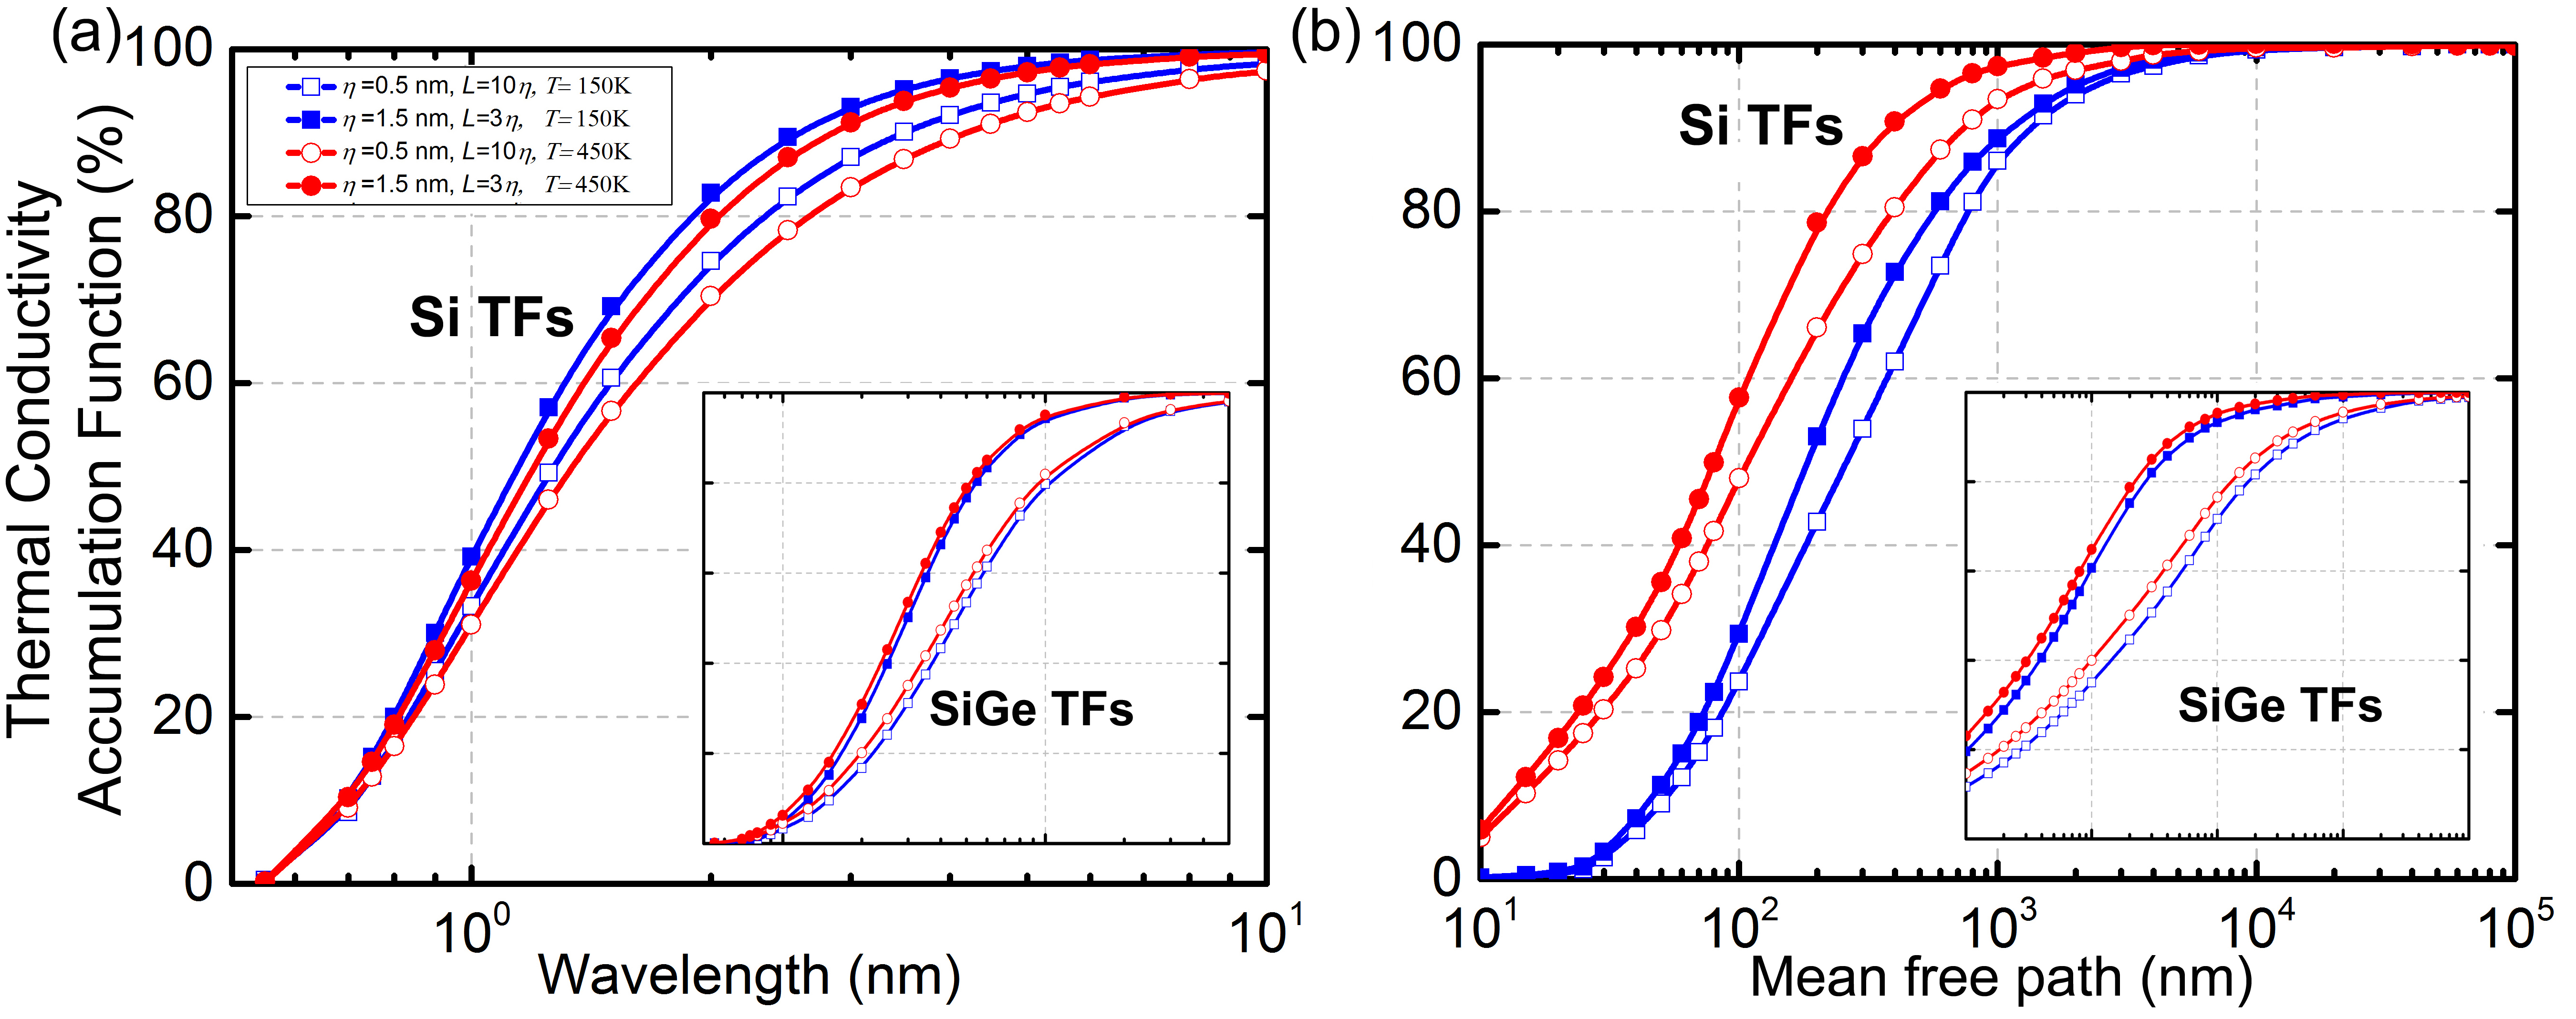
\includegraphics[width=\textwidth]{/ch2/Figure-TF-Spectra2.jpg}
  \caption{Dependence of the accumulation functions on temperature (450 K in red lines and 150 K in blue lines) for Si thin film (\sige{0.90}{0.10}, insets) of thickness \gls{t} = 100nm and rough (\gls{eta} = 1.5 nm, \gls{cl} = 3\gls{eta} filled symbols) and smooth (\gls{eta} = 0.5 nm, \gls{cl} = 10\gls{eta}, open symbols) boundaries. The accumulation function is presented across phonon (a) wavelengths and (b) mean-free-paths.}
  \label{fig:ch2-tf-spectra-2}
\end{figure}
\par These results show how the specific surface properties and temperatures can significantly modify the thermal conductivity accumulation, opening a way forward to the rational design of the semiconductor-air interfaces, which can be utilized to tailor the desired thermal transport properties in nanostructures. This principle of purposely modified phonon transport properties is illustrated in \Cref{fig:ch2-tf-spectra-3}, where surface properties, thicknesses, and alloying are used to modulate the thermal energy distribution of silicon. Introduction of alloy atoms creates a shift towards a large-wavelength energy spectra (i.e., red-shift). A film with a perfectly smooth surface would exhibit the energy spectra of the bulk alloy but surface roughening and thickness variations can be made to blue-shift towards shorter wavelength spectra. A rougher interface and a smaller film size both favor blue-shift of wavelength spectra as the effects of boundary scattering are more pronounced. As a result, the amount of thermal energy carried by phonons with wavelengths in the range 1–10 nm can be designed to be from $\sim$ 30\% to 90\%.
%Spectra TF 3
\begin{figure}[hbt]
  \centering 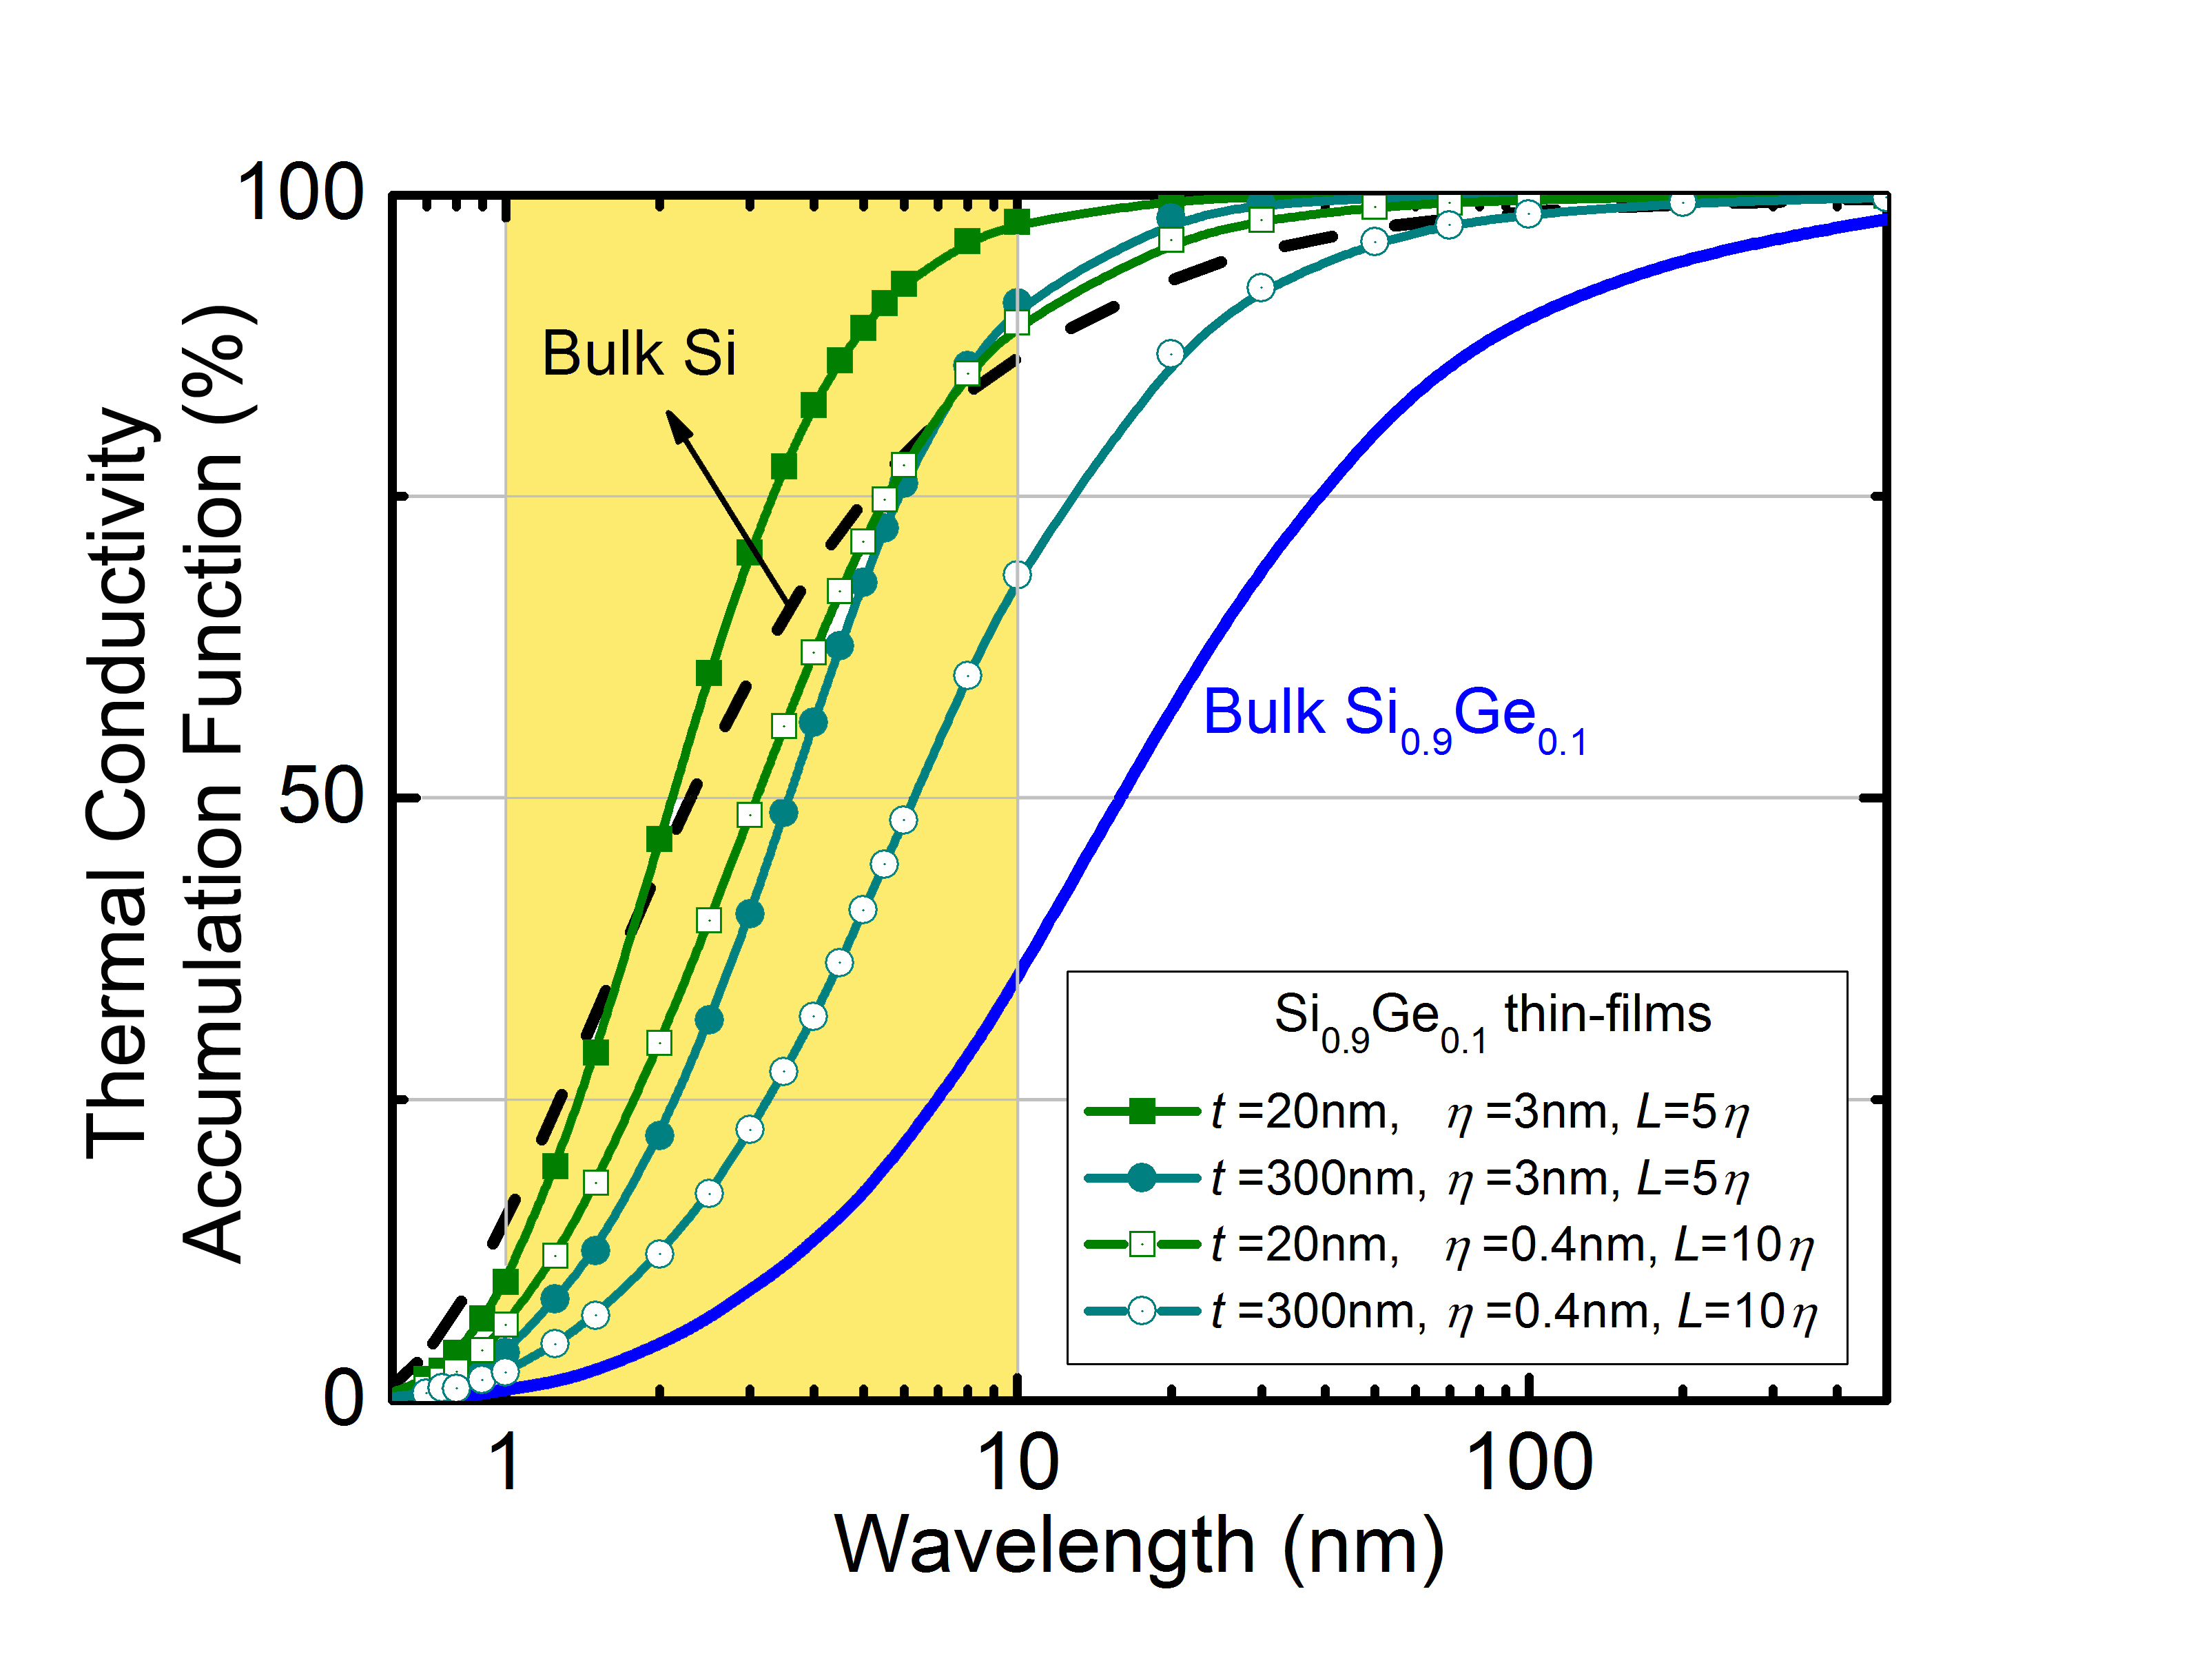
\includegraphics[width=\textwidth]{/ch2/Figure-TF-Spectra3.jpg}
  \caption{Thermal conductivity accumulation (or heat spectra) modification in \sige{0.90}{0.10} thin-films at room temperature by varying surface properties and thicknesses. Bulk Si and \sige{0.90}{0.10} accumulation functions are presented as reference. The proportion of heat carried by phonons with wavelengths \gls{wl} = 1–10 nm can be made to vary from 30\% to 90\% by tuning phonon scattering.}
  \label{fig:ch2-tf-spectra-3}
\end{figure}

\section{Estimating the Importance of Phonon Confinement}
It is important to highlight that advances in manufacturing techniques have enabled the production of thin films with very small thicknesses. At very small length scales, phonon quantum effects can become important and can play an important role in heat transport \cite{RN205,RN153}. Using our surface scattering and heat transport model, we show the emergence and impact of phonon quantum confinement effects \cite{RN139} in Si and SiGe thin-films. We note that a similar function can be defined for nanowires \cite{ownNW}. The introduction of the film boundaries allows for the creation of spatially confined phonons which behave as standing waves in the direction normal to the surfaces. We define a Confinement Contribution Fraction (CCF) to quantify the potential influence of phonon confinement in thin-films. CCF is calculated as the proportion of thermal energy conducted by phonons which can satisfy the confinement criteria in a nanostructure. Note that confined phonons may show modified transport properties, such as group velocities, due to coherent interference and resultant modified dispersion relations. Thus, a thin-film whose thermal conductivity values can be highly influenced by phonon quantum confinement exhibit a higher CCF value. The conditions that need to be satisfied by a phonon to be confined are twofold. First criterion requires mean-free-paths \gls{mfp} be sufficiently long so that phonons can effectively ``see" the two film boundaries. Second, Si-air interfaces (which behave as boundaries of infinite potential for the phonons) restrict and quantize the allowed wave vectors propagating in the direction normal to the surfaces when brought close together. Phonons with wavelengths larger than 2\gls{t} $\cos\theta$ (where \gls{t} is the thickness, and \gls{theta} the angle with surface normal) are entirely transformed to non-propagating modes, while larger k-space phonons can still propagate but subject to confinement effects \cite{book_Zangwill}. On the basis of this limiting condition, we define the minimum [i.e., $\lambda_1>2t\cos\theta$] and upper threshold [$\lambda_2>(2t\cos\theta)/5$] of the impact of confinement effects on heat conduction in Si and SiGe thin films and calculate the Confinement Contribution Fractions, CCF\textsubscript{min} and CCF\textsubscript{max}, respectively [\Cref{fig:ch2-confinement}(a) and (b)]. Note that the condition for $\lambda_2$ is an estimate to gauge the maximum influence of confinement in nanostructures based on the fact that the allowed wavelengths are discrete and quantized in a nanostructure. Specifically, the first five quantized values are separated to a larger degree than the subsequent values, and therefore, the middle-point of an order of magnitude change is taken as a measure of strong confinement effects (i.e., $\lambda_2$). Solid (CCF\textsubscript{min}) and dotted (CCF\textsubscript{max}) lines have similar values at large thicknesses because of the inability of the phonons to see the two interfaces due to phonon-phonon scattering. For intermediate thicknesses, the two lines separate as the wavelength conditions begin to dictate the possibility of confinement. At small thicknesses, even though a wide range of phonons can satisfy the wavelength confinement conditions, only a limited number of them with sufficiently large mean-free-paths (to form a standing wave) can show confinement. In general, rougher interfaces exhibit smaller confinement influenced conductivity as shown by smaller CCF values for \gls{eta} = 0.5 nm than \gls{eta} = 0.25 nm (\gls{cl} = 10\gls{eta} for both cases) and the contribution of phonon confinement effects reduces (marked by decreasing CCF) with increasing thicknesses. An analysis for temperature shows that confinement effects are significantly enhanced at lower temperatures as longer wavelength (and mean-free-path) phonons carry more heat. For example, in Si thin films of roughness 0.5 nm and \gls{cl} = 5 nm, CCF = 0.02 at room temperatures for 10 nm thick structures in contrast to CCF = 0.13 at 20 K. We note that for thicker (\gls{t}$\sim$30 nm) Si thin films at room temperatures, CCF values for typical interfacial roughness (\gls{eta} = 0.5 nm) quantitatively indicate that phonon confinement effects are negligible, while for very smooth interfaces (\gls{eta} = 0.25 nm) these effects are shown to be small. Similar trends with temperature are observed in the case of \sige{0.90}{0.10} alloyed thin films (CCF = 0.05 and 0.18 at 300 K and 20 K, respectively). Importantly, the use of only 10\% Ge makes the alloyed thin films a better candidate to explore confinement as compared to pure Si. This is due to the efficient scattering of small wavelengths by heavier atoms of Ge in the crystalline lattice of Si which shifts the thermal conductivity accumulation function towards larger wavelength thermal phonons as compared to crystalline Si.
\begin{figure}[hbt]
  \centering 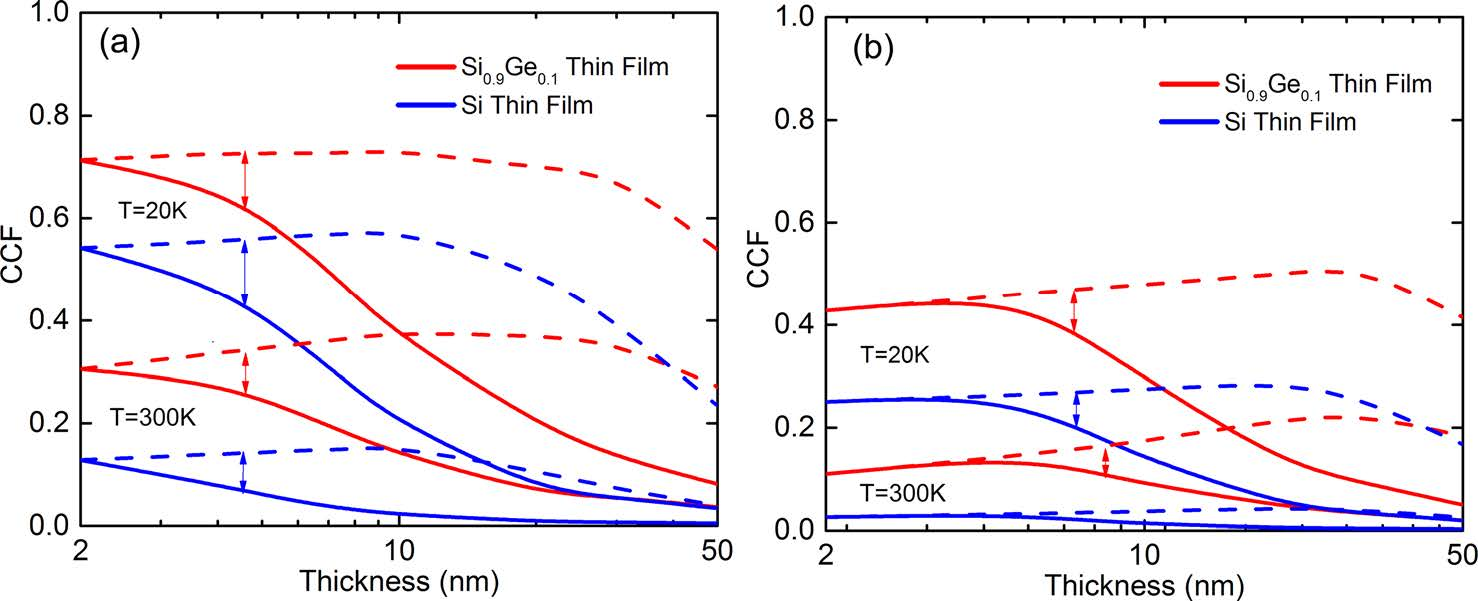
\includegraphics[width=\textwidth]{/ch2/Figure-TF-confinement.jpg}
  \caption{Confinement Contribution Functions (CCF) calculated at room temperature and \gls{T} = 20 K for thin films with correlation lengths \gls{cl} = 10\gls{eta} and roughness (a) \gls{eta} = 0.25 nm (b) \gls{eta} = 0.5 nm. CCF\textsubscript{min} (solid line) is the minimum contribution of confined modes to conductivity due to mode conversion in spatially confined nanostructures, while CCF\textsubscript{max} (dashed line) gives an upper threshold to this contribution. Double arrows are used as guide to the eyes.}
  \label{fig:ch2-confinement}
\end{figure}

\section{Summary}
The absence of rigorous theoretical descriptions for phonon-surface interaction have precluded the creation of truly predictive models which rely on experimentally quantifiable descriptors and embody key physics of phonon-surface scattering. To address this issue, we introduced an approach to predict heat transport in nanowires and thin films by considering the reduction in phonon mean-free-paths via the Beckmann-Kirchhoff rough surface scattering theory along with rough surface shadowing. This approach considers all critically relevant physical variables behind the phonon interface interactions and phonon transport viz. phonon momentum, angle of incidence of phonons with the surface, surface roughness and surface correlation length. We developed a model that could determine the energy distribution using the thermal conductivity accumulation function across phonon mean-free-paths and wavelengths in Si and SiGe nanowires and thin films with varying surface conditions. The applicability of our model is demonstrated by the excellent agreement with a range of experimental measurements. These results help to fundamentally understand heat transport at the nanoscale and provide a route to accurately establish the transport mechanisms with the use of experimentally quantifiable parameters.	